\documentclass[a4paper,12pt]{extarticle}

%---------------- PACKAGES ----------------
\usepackage[utf8x]{inputenc}
\usepackage[T1]{fontenc}
\usepackage[french]{babel}
\usepackage{amsmath}
\usepackage{xcolor}
\usepackage{graphicx}
\usepackage{fancyhdr}
\usepackage{hyperref}
\usepackage{url}
\usepackage{booktabs}
\usepackage[hypcap=false]{caption}
\usepackage{float}
\usepackage{listings}
\usepackage{tabularx}
\usepackage{booktabs}
\usepackage{array}
\usepackage{minted}
\usepackage[protrusion=true,expansion=false]{microtype}


\definecolor{bgcolor}{RGB}{110, 90, 109}
\definecolor{codegreen}{RGB}{152, 195, 121}
\definecolor{codeblue}{RGB}{97, 175, 239}
\definecolor{codewhite}{RGB}{248, 248, 242}

\lstdefinestyle{terminal}{
    backgroundcolor=\color{bgcolor},
    basicstyle=\ttfamily\small\color{codewhite},
    keywordstyle=\color{codeblue},
    commentstyle=\color{codegreen},
    showstringspaces=false,
    breaklines=true,
    frame=single,
    rulecolor=\color{black}
}


%---------------- HEADER STYLE ----------------
\setlength{\headheight}{14.5pt}
\addtolength{\topmargin}{-4.5pt}

\pagestyle{fancy}
\fancyhf{}
\fancyhead[L]{HESTIM}
\fancyfoot[C]{\thepage}
\renewcommand{\headrulewidth}{0.4pt}
\renewcommand{\footrulewidth}{0.4pt}

%---------------- PAGE DE GARDE : EN-TÊTE DÉDIÉ ----------------
\fancypagestyle{coverpage}{%
    \fancyhf{}%
    \fancyhead[L]{
\includegraphics[height=1cm]{images/1.png}}%
    \fancyhead[R]{\small\textsc{HESTIM}}%
    \renewcommand{\headrulewidth}{0.4pt}%
    \renewcommand{\footrulewidth}{0pt}%
}

\begin{document}

%================================================
% PAGE DE TITRE
%================================================
\begin{titlepage}
\thispagestyle{coverpage}
\centering
\vspace*{0.25cm}

{\Large \textsc{HESTIM Engineering \& Business School}}\\[0.15cm]
{\large Rapport de stage}\\[0.4cm]
\textsc{\large Filière : Génie Informatique et Intelligence Artificielle}\\[0.6cm]

\rule{\linewidth}{0.6mm}\\[0.4cm]
{\Large \textbf{\textsc{Conception et développement d'une plateforme
    de commande et d'interaction autonome\\[0.2cm]
    pour un robot de service Android}}}\\[0.4cm]
\rule{\linewidth}{0.6mm}

\vfill
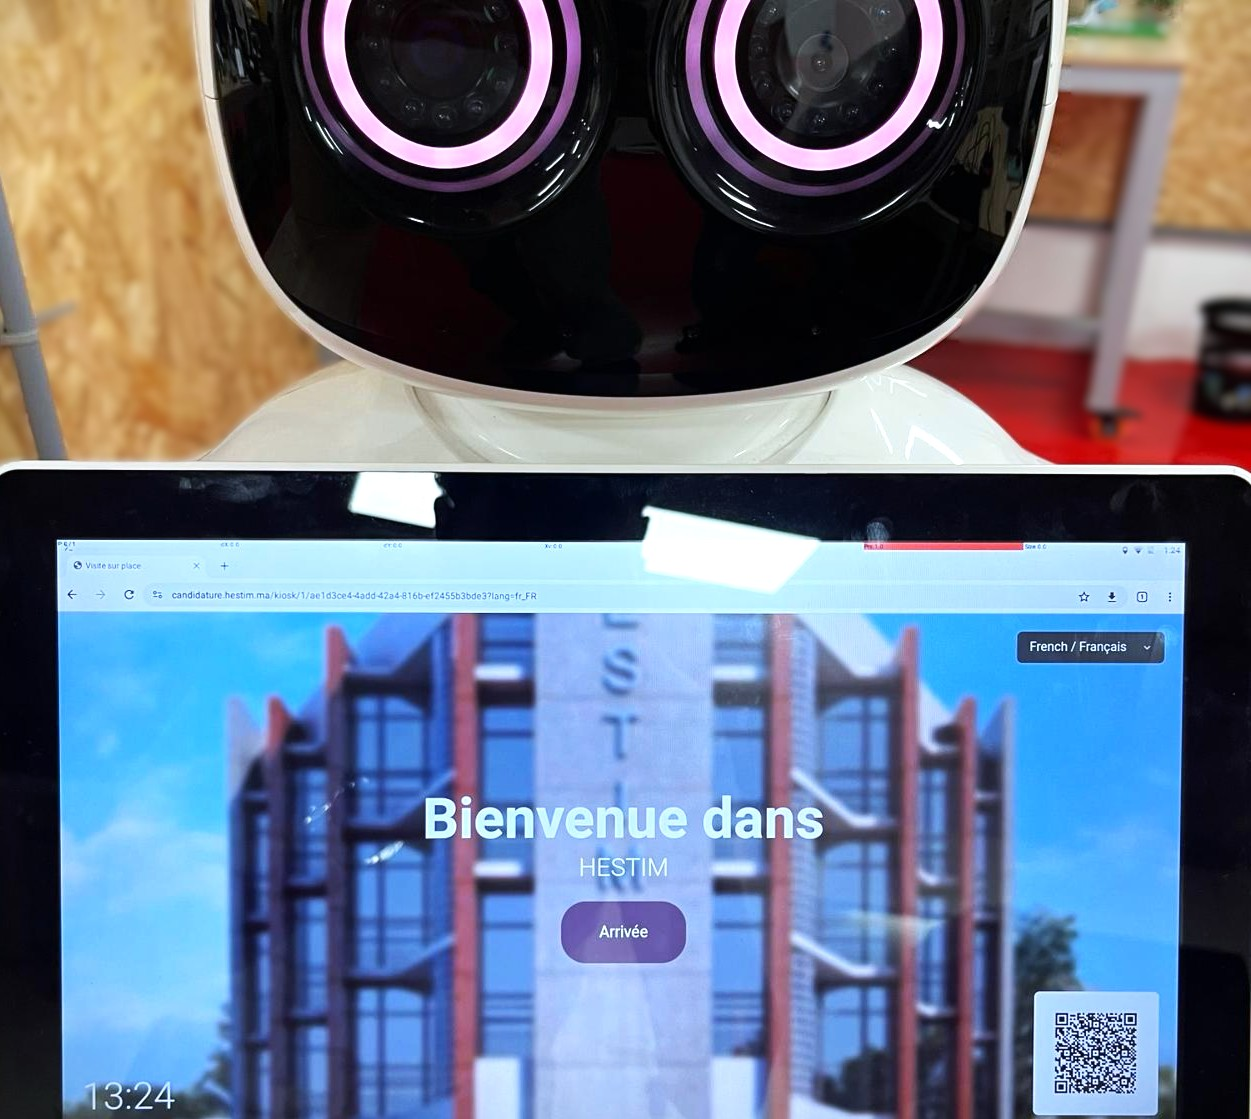
\includegraphics[width=0.48\textwidth]{images/cybel1.jpeg}
\vfill

% Auteurs / Encadrant
    \begin{minipage}{0.45\textwidth}
        \begin{flushleft}\large
            \emph{Réalisé par :}\\[0.2cm]
            Claudia \textsc{LUSAMOTE KIMFUTA}\\
        \end{flushleft}
    \end{minipage}
    \hfill
    \begin{minipage}{0.45\textwidth}
        \begin{flushright}\large
            \emph{Encadrante pédagogique :}\\[0.2cm]
            Mme \textsc{MESKINI} Fatime Zahra\\[0.35cm]
            \emph{Encadrant industriel :}\\[0.2cm]
            M \textsc{TULA} Sridath\\[0.3cm]
        \end{flushright}
    \end{minipage}\\[0.5cm]

\rule{\linewidth}{0.3mm}\\[0.35cm]
Classe : \textsc{\normalsize 1\textsuperscript{ère} du cycle d'ingénieur}\\[0.2cm]
\textbf{Année universitaire : 2025 - 2026}
\vspace*{0.2cm}

\end{titlepage}

%================================================
% PAGES PRÉLIMINAIRES
%================================================
\pagenumbering{roman}

\section*{\centering REMERCIEMENTS}
\addcontentsline{toc}{section}{REMERCIEMENTS}

Nous tenons à exprimer notre profonde gratitude à notre encadrant, Dr. Sridath Tula, pour son accompagnement, sa disponibilité et ses précieux conseils tout au long de la réalisation de ce projet. Son expertise, ses orientations et son soutien constant ont grandement contribué à l'aboutissement de ce travail.

Nous adressons également nos sincères remerciements à l'ensemble du corps professoral ainsi qu'au personnel administratif et technique de HESTIM pour la qualité de la formation dispensée, leur professionnalisme et les moyens mis à notre disposition tout au long de notre parcours académique.

Nous remercions particulièrement les responsables de la filière Génie Informatique pour leur encadrement et les connaissances qu'ils nous ont transmises au cours de ces années d'études, nous permettant d'acquérir les compétences nécessaires à la réalisation de ce projet.

Nous souhaitons également exprimer notre reconnaissance envers toutes les personnes qui, de près ou de loin, ont contribué à la réussite de ce travail par leurs conseils, leurs encouragements ou leur soutien.

Enfin, nous adressons nos plus sincères remerciements à nos familles et à nos proches pour leur patience, leur confiance et leurs encouragements constants. Leur soutien moral a été une source de motivation essentielle tout au long de cette expérience.

Ces remerciements témoignent de notre reconnaissance envers toutes les personnes qui ont contribué à la réussite de ce projet et à l'enrichissement de notre parcours académique et personnel.

\newpage
\section*{\centering RÉSUMÉ}
\addcontentsline{toc}{section}{RÉSUMÉ}

Les robots de service mobiles sont généralement livrés avec un écosystème logiciel fermé :
application propriétaire, absence de documentation et de protocole de communication publié.
Ce constat limite toute personnalisation par l'utilisateur final. Le projet \textsc{Cybel}, mené
dans le cadre d'un stage à HESTIM, vise à concevoir une plateforme de commande et
d'interaction indépendante pour un robot de réception mobile CIOT TY1251D-03195, composé d'un
châssis de navigation sous ROS et d'un \emph{« upper body »} Android.

La démarche adoptée repose sur une rétro-ingénierie incrémentale et non destructive du protocole
de communication interne du robot : balayage des services réseau exposés, introspection des
topics et services ROS via \texttt{rosbridge}/\texttt{rosapi}, et vérification systématique de
l'effectivité de chaque commande avant de la considérer comme fonctionnelle. Sur cette base, une
architecture en trois couches a été conçue~:
\begin{itemize}
    \item un SDK Python proposant une implémentation simulée (\emph{mock}) et une implémentation
    réelle interchangeables ;
    \item une API FastAPI (REST~+~WebSocket) ;
    \item une interface web Vite/TypeScript opérateur ;
\end{itemize}
complétée par une interface visiteur kiosque (\texttt{frontend-kiosk/}) et deux applications
Android natives légères (\texttt{CybelTTSBridge}, \texttt{CybelVisitorKiosk}).

À ce stade du stage, la connectivité avec le robot est établie, le protocole de télémétrie, de
commande de vitesse et de navigation autonome a été reconstruit et intégré, la synthèse vocale
(TTS) fonctionne via une application Android dédiée déclenchée par \texttt{am broadcast}, une
interface opérateur complète (carte SLAM, LiDAR, visiteurs détectés, gestion du parcours de
visite, arrêt d'urgence pendant une visite) est opérationnelle, et un déploiement embarqué sur
Termux (\emph{backend lite} + kiosque) est validé sur la tablette. L'interface visiteur a été
recentrée sur une visite guidée autonome du laboratoire : huit arrêts synchronisés depuis
\texttt{data/knowledgeV2-lab.json} vers \texttt{data/lab\_tour.json}, navigation par coordonnées
(\texttt{/navi\_goal}) et annonces vocales séquentielles.

Ce rapport présente le contexte, la problématique, l'état de l'art, la conception, la
méthodologie, l'implémentation réalisée, les résultats obtenus, ainsi qu'une analyse critique des
limites et perspectives du projet.

\bigskip
\noindent\textbf{Mots-clés :} robotique de service, rétro-ingénierie de protocole, ROS,
rosbridge, FastAPI, interface homme-robot, navigation autonome, synthèse vocale, Termux, WebView
Android.
\newpage
\section*{\centering ABSTRACT}
\addcontentsline{toc}{section}{ABSTRACT}

Mobile service robots are typically delivered with a closed software ecosystem: a proprietary
application, no documentation, and no published communication protocol. This severely limits any
customization by the end user. The \textsc{Cybel} project, carried out as part of a final-year
internship at HESTIM, aims to design an independent control and interaction platform for a CIOT
TY1251D-03195 mobile reception robot, consisting of a ROS-based navigation chassis and an Android
\emph{« upper body »}.

The approach adopted relies on an incremental, non-destructive reverse engineering of the robot's
internal communication protocol: scanning of exposed network services, introspection of ROS
topics and services via \textbf{rosbridge}/\textbf{rosapi}, and systematic verification of the
actual effect of each command before considering it functional. On this basis, a three-layer
architecture was designed:
\begin{itemize}
    \item a Python SDK offering interchangeable simulated (\emph{mock}) and real implementations;
    \item a FastAPI backend (REST~+~WebSocket);
    \item a Vite/TypeScript operator web interface;
\end{itemize}
complemented by a visitor kiosk interface (\texttt{frontend-kiosk/}) and two lightweight native
Android applications (\texttt{CybelTTSBridge}, \texttt{CybelVisitorKiosk}).

At this stage of the internship, connectivity with the robot has been established; the
telemetry, speed control, and autonomous navigation protocols have been reverse-engineered and
integrated; text-to-speech (TTS) works through a dedicated Android application triggered via
\texttt{am broadcast}; a complete operator interface (SLAM map, LiDAR, detected visitors, tour
management, emergency stop during a visit) is operational; and an embedded deployment on Termux
(\emph{backend lite} + kiosk) has been validated on the tablet. The visitor interface has been
refocused on an autonomous guided tour of the laboratory: eight stops synchronized from
\texttt{data/knowledgeV2-lab.json} to \texttt{data/lab\_tour.json}, coordinate-based navigation
(\texttt{/navi\_goal}), and sequential voice announcements.

This report presents the context, problem statement, state of the art, design, methodology,
implementation carried out, results obtained, as well as a critical analysis of the project's
limitations and perspectives.

\bigskip
\noindent\textbf{Keywords:} service robotics, protocol reverse engineering, ROS, rosbridge,
FastAPI, human–robot interface, autonomous navigation, text-to-speech, Termux, Android WebView.

%---------------- SOMMAIRE ----------------
\newpage
\tableofcontents

%---------------- LISTES ----------------
\newpage
\listoffigures

\newpage
\listoftables

\newpage
\newpage
\section*{\centering LISTE DES ABRÉVIATIONS}
\addcontentsline{toc}{section}{LISTE DES ABRÉVIATIONS}

\begin{description}
    \item[ADB] Android Debug Bridge
    \item[API] Application Programming Interface (Interface de programmation applicative)
    \item[APK] Android Package (format d'installation des applications Android)
    \item[DHCP] Dynamic Host Configuration Protocol
    \item[HRI] Human-Robot Interaction (Interaction Homme-Robot)
    \item[HTTP] HyperText Transfer Protocol
    \item[IHM] Interface Homme-Machine
    \item[IP] Internet Protocol
    \item[JSON] JavaScript Object Notation
    \item[LiDAR] Light Detection and Ranging
    \item[MQTT] Message Queuing Telemetry Transport
    \item[REST] Representational State Transfer
    \item[RK3399] Référence du système sur puce (SoC) équipant la tête Android du robot
    \item[ROS] Robot Operating System
    \item[rosbridge] Composant ROS exposant les topics et services ROS via WebSocket
    \item[rosapi] Service ROS d'introspection des topics, services et types de messages
    \item[SDK] Software Development Kit (Kit de développement logiciel)
    \item[SLAM] Simultaneous Localization and Mapping (Cartographie et localisation simultanées)
    \item[SoC] System on Chip (Système sur puce)
    \item[TCP/IP] Transmission Control Protocol / Internet Protocol
    \item[TTS] Text-To-Speech (Synthèse vocale)
    \item[UML] Unified Modeling Language
    \item[WebSocket] Protocole de communication bidirectionnelle en temps réel sur TCP
\end{description}


%================================================
% CORPS DU RAPPORT
%================================================
\clearpage
\pagenumbering{arabic}

\pagestyle{fancy}

%================ INTRODUCTION =================
\section*{\centering INTRODUCTION GÉNÉRALE}
\addcontentsline{toc}{section}{INTRODUCTION GÉNÉRALE}

\indent Les robots de service autonomes occupent une place croissante dans les environnements professionnels accueil, guidage, télépresence grâce à la maturité des technologies de navigation autonome et d'interaction homme-robot. Ces robots sont cependant généralement livrés avec un écosystème logiciel fermé : application propriétaire, protocole non documenté, absence d'API publique. Cette fermeture limite fortement la capacité des utilisateurs à adapter leur comportement à des besoins spécifiques.

C'est dans ce contexte que s'inscrit le robot de réception mobile \textbf{CIOT TY1251D-03195}, mis à disposition par HESTIM Engineering \& Business School dans le cadre d'un stage de fin d'année. Composé d'un châssis de navigation sous ROS et d'une tête Android assurant l'interface visiteur, ce robot dépend entièrement d'une application propriétaire pour laquelle aucune documentation n'est disponible. Le projet \textbf{CYBEL}, objet de ce rapport, vise à concevoir une plateforme logicielle indépendante permettant de superviser, piloter et faire interagir ce robot sans recourir à l'application d'origine.

La problématique du stage est donc double : comment établir une communication fiable avec un système robotique fermé dont ni le protocole, ni les points d'accès réseau ne sont connus, et comment construire à partir de cette compréhension reconstruite une solution de contrôle robuste et extensible ? Le stage, d'une durée de trois à quatre mois, poursuit ainsi deux objectifs : procéder à une rétro-ingénierie méthodique du protocole de communication interne du robot, puis développer sur cette base une plateforme de commande complète, incluant une interface opérateur, une interface visiteur et des fonctionnalités d'interaction tactile et vocale. La démarche adoptée repose sur une approche itérative et prudente, où chaque hypothèse sur le fonctionnement du robot est systématiquement vérifiée avant d'être considérée comme acquise.

Le présent rapport restitue cette démarche en sept chapitres : présentation de l'entreprise d'accueil, analyse du besoin et étude préalable, état de l'art, analyse et conception du système CYBEL, méthodologie et planification, réalisation et implémentation, puis validation, résultats et analyse critique, avant une conclusion générale dressant le bilan du stage et ses perspectives.


%================================================
% PARTIE 1 : CONTEXTE ET ANALYSE
%================================================
\newpage
\section{Présentation de l'entreprise}

L'HESTIM Engineering School (Hautes Études des Sciences et Techniques de
l'ingénierie et du Management) est un établissement privé d'enseignement
supérieur basé à Casablanca, au Maroc. Fondée en 2006, elle forme chaque
année plusieurs centaines d'étudiants dans les domaines de l'ingénierie et
du management. HESTIM fonctionne comme une entreprise de formation et de
services académiques, structurée pour répondre aux besoins croissants des
secteurs industriels et technologiques au Maroc et à l'international.

\begin{figure}[H]
	\centering
	
\includegraphics[width=0.35\textwidth]{images/1.png}
\end{figure}

\subsection{Activité principale et services}

HESTIM propose des formations d'ingénieurs et de managers dans plusieurs
spécialités, notamment :

\begin{itemize}
	\item Génie Informatique et Intelligence Artificielle
	\item Génie Industriel et Logistique
	\item Génie Civil et Travaux Publics
	\item Management et Administration des Affaires
\end{itemize}

L'établissement offre des programmes d'enseignement initial, de formation
continue et de doubles diplômes, en partenariat avec des universités et
écoles étrangères. Il met également à disposition des laboratoires
techniques et des équipements modernes : robots collaboratifs, capteurs
3D, robots de service Android ainsi que des services de recherche
appliquée pour accompagner l'innovation.

\subsection{Organisation interne}

HESTIM est organisée autour de plusieurs pôles clés :

\begin{itemize}
	\item \textbf{Pôle pédagogique}, qui regroupe les départements de
	formation spécialisés.
	\item \textbf{Pôle administratif}, qui assure la gestion des étudiants
	et des relations avec les entreprises partenaires.
	\item \textbf{Pôle recherche et développement}, qui coordonne les
	projets innovants menés en collaboration avec des entreprises ou dans
	le cadre de projets étudiants, dont le projet CYBEL fait partie.
\end{itemize}

\subsubsection{Organigramme de l'HESTIM}

Pour illustrer la structure interne de l'HESTIM et mieux situer notre
projet dans son environnement, voici un organigramme simplifié de
l'établissement.

\begin{center}
	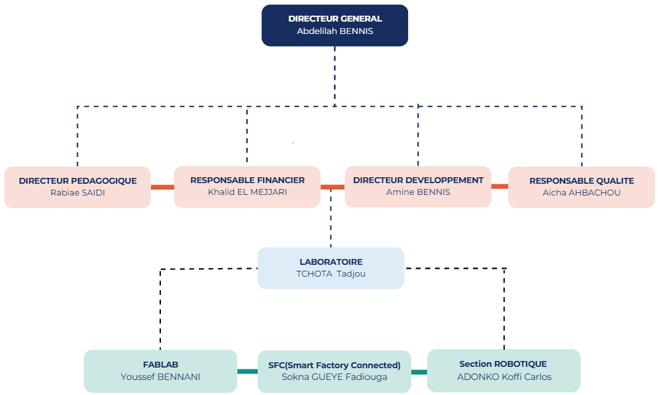
\includegraphics[width=0.9\textwidth]{images/organigramme.png}
	\captionof{figure}{Organigramme de l'HESTIM}
\end{center}

\subsection{Positionnement dans le secteur}

HESTIM s'est imposée comme l'une des écoles d'ingénierie et de management
les plus reconnues au Maroc. Elle bénéficie d'une réputation solide grâce à :

\begin{itemize}
	\item la qualité de ses formations orientées vers les besoins concrets
	du marché ;
	\item ses nombreux partenariats avec des acteurs industriels nationaux
	et internationaux ;
	\item son engagement dans l'innovation pédagogique et technologique,
	notamment dans les domaines de la robotique et de l'intelligence
	artificielle.
\end{itemize}

HESTIM accueille un public varié, marocain et étranger, et cible des
secteurs clés comme l'industrie, les technologies de l'information, le BTP
et la logistique.

\subsection{Valeurs et engagements}

HESTIM place l'innovation, la qualité pédagogique et l'ouverture
internationale au cœur de sa stratégie. L'école vise à former des
ingénieurs et managers capables de répondre aux défis actuels et futurs de
l'industrie, avec un fort accent sur l'éthique, l'esprit d'équipe et
l'adaptabilité aux évolutions technologiques.

\subsection{Lien avec notre stage}

Le stage s'est déroulé au sein de HESTIM, considérée comme l'établissement
d'accueil, car l'école offre un cadre idéal pour mettre en pratique les
connaissances en génie informatique et en intelligence artificielle. La
présence sur site du robot de service Android \textit{CIOT TY1251D-03195} a
permis d'expérimenter directement sur le matériel cible.

Le présent rapport documente la plateforme CYBEL, développée par
Claudia Lusamote Kimfuta ; Ghassane Khalifi a mené en parallèle un travail
complémentaire sur un module chatbot (branche dédiée du dépôt GitHub), non
détaillé dans les chapitres techniques suivants. Grâce aux équipements du
FabLab et à l'environnement de travail du laboratoire, ce stage a permis de
mobiliser des compétences en rétro-ingénierie de protocoles, en
développement d'API et en interfaces homme-robot, en adéquation avec le
programme de la filière Génie Informatique.

\subsection{Conclusion}

La présentation de l'HESTIM Engineering School met en évidence un
environnement académique et technologique favorable à la réalisation de
projets innovants. Sa structure, ses équipements et en particulier la
disponibilité du robot \textit{CIOT TY1251D-03195} et ses formations orientées vers
l'industrie~4.0 ont permis de mener ce stage dans des
conditions optimales, alliant rigueur académique et mise en situation
professionnelle réelle.

\newpage
\section{Analyse du besoin et étude préalable}

Ce chapitre présente le contexte général du projet CYBEL ainsi que l'analyse
du besoin ayant conduit à la définition de la solution proposée. Il met en
évidence l'architecture du système étudié, la problématique associée, les
objectifs du projet ainsi que le cahier des charges fonctionnel et technique.

\subsection{Contexte du projet}

\subsubsection*{Présentation du robot CIOT TY1251D-03195}

Le robot étudié est un \textbf{robot de réception mobile} commercialisé sous la
référence \textbf{CIOT TY1251D-03195} illustré sur la  figure~\ref{fig:robot}. Il est composé de deux sous-systèmes
matériels distincts, reliés en interne :

\begin{itemize}
    \item un \textbf{châssis de navigation} fonctionnant sous \textbf{Linux
    embarqué avec ROS}, responsable de la localisation (SLAM), de la planification
    de trajectoire (\texttt{move\_base}) et de l'exécution des commandes de
    mouvement ;
    \item un \textbf{\og upper body \fg{} Android 7.1} (SoC RK3399, 2 Go de RAM,
    16 Go de stockage), équipé d'un écran tactile 15,6" (1920×1080), de caméras
    (reconnaissance faciale, surveillance) et de haut-parleurs, qui héberge
    l'application propriétaire d'accueil et l'interface utilisateur standard du
    robot.
\end{itemize}

Le robot dispose d'un point d'accès WiFi propre (\texttt{TY1251D-03195})
permettant à un poste externe de rejoindre son réseau local. La topologie
réseau s'est révélée plus complexe que ne le laissait supposer une simple
architecture à deux hôtes : le châssis est joignable à l'adresse fixe
\texttt{10.42.0.1}, tandis que la tête Android obtient une adresse variable
par DHCP sur un second segment \texttt{172.16.0.0/16} une première IP
documentée (\texttt{172.16.0.88}) s'est révélée périmée en cours de projet.
Les deux sous-systèmes sont par ailleurs reliés en interne par une liaison
filaire \texttt{eth0} sur le segment \texttt{192.168.20.0/24}
(\texttt{192.168.20.1} pour la tête, \texttt{192.168.20.22} pour le châssis),
indépendante du réseau WiFi exposé à l'extérieur.

\begin{center}
    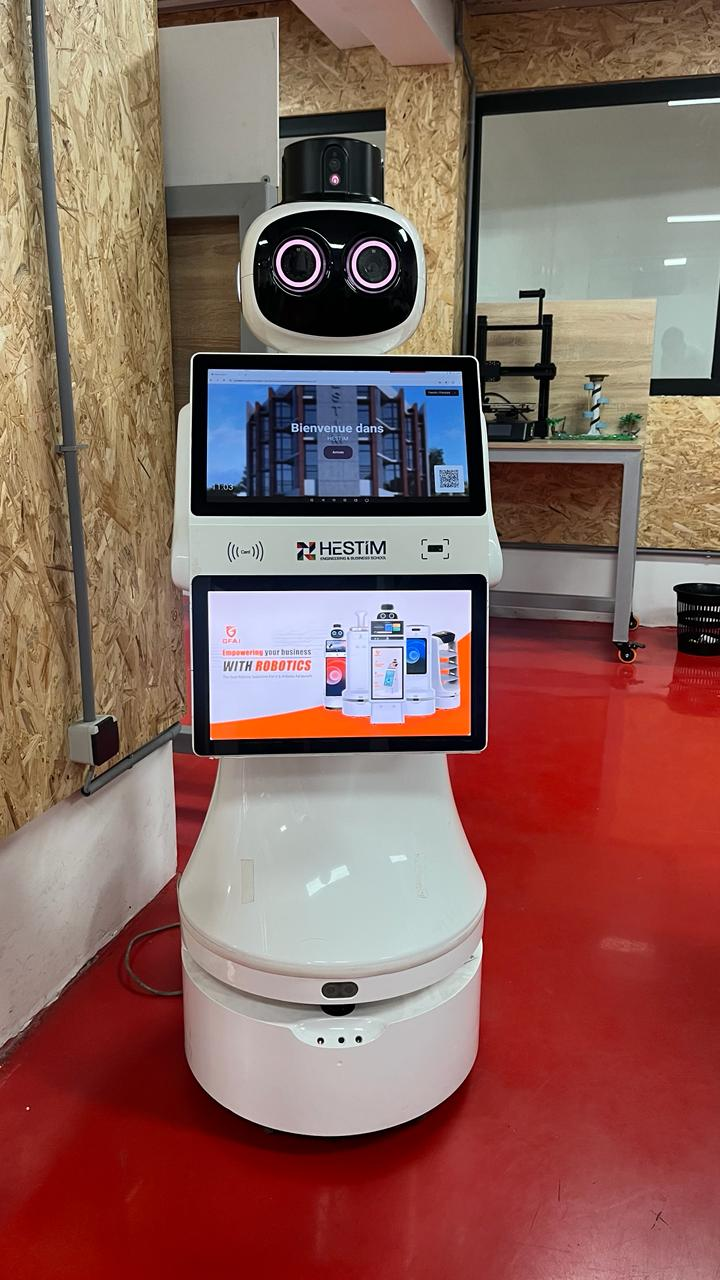
\includegraphics[width=0.4\textwidth]{images/cybel.jpeg}
    \captionof{figure}{Robot CIOT TY1251D-03195 "CYBEL"}
    \label{fig:robot}
\end{center}

\subsubsection*{Architecture générale du robot}

Vue dans son ensemble, l'architecture du système peut se lire en quatre
couches superposées, illustrées en figure~\ref{fig:archi_robot} : une couche
de présentation et d'interaction, une couche applicative et API, une couche
de communication et de services réseau, et une couche matérielle.

\paragraph{Couche de présentation et d'interaction (couche supérieure):}Au sommet de l'architecture se trouve la couche de présentation, qui regroupe
l'ensemble des interfaces utilisateur permettant d'interagir avec le robot.
On y distingue trois composants principaux : l'\textbf{application
propriétaire Android}, considérée comme une boîte noire non documentée et
hors du périmètre du projet ; l'\textbf{interface opérateur web (CYBEL)},
développée dans le cadre du projet et permettant le contrôle et la
supervision du robot ; et l'\textbf{interface visiteur (mode kiosque)},
dédiée aux interactions simplifiées dans un contexte public. Cette couche
constitue le point d'entrée principal des interactions homme-machine et
repose sur des échanges réseau vers les couches inférieures, notamment via
HTTP et WebSocket. Deux composants complémentaires y sont également présents
côté Android : un module de \textbf{synthèse vocale (TTS natif)}, permettant
les retours audio du robot, et un mode \textbf{WebView kiosque}, utilisé pour
des interactions simplifiées embarquées.

\paragraph{Couche applicative et API (couche intermédiaire):}
La deuxième couche correspond à la logique applicative centrale du système,
matérialisée par l'\textbf{API CYBEL développée en FastAPI}. Cette API joue
un rôle d'orchestrateur entre les interfaces utilisateur et les mécanismes
de communication avec le robot : elle expose des endpoints REST ainsi que
des canaux WebSocket pour la supervision en temps réel. Elle est alimentée
par deux types de clients un \textbf{SDK Python en mode réel}, qui assure
la communication directe avec le robot, et un \textbf{SDK Python en mode
simulé (\textit{mock})}, permettant le développement et les tests
indépendamment du matériel. Ces deux modes convergent vers une interface
commune abstraite (\texttt{RobotBackend}), garantissant la continuité
fonctionnelle entre simulation et exécution réelle.

\paragraph{Couche de communication et de services réseau:}
La troisième couche représente les interfaces réseau exposées par le robot
et utilisées comme points d'accès aux fonctionnalités internes. Elle
comprend plusieurs services distincts : \textbf{rosbridge} (WebSocket, port
9090), permettant l'envoi et la réception de messages ROS au format JSON ;
\textbf{rosapi}, utilisé pour l'introspection des topics, services et
abonnés ROS ; \textbf{MQTT} (port 1883), employé pour la communication
événementielle et la télémétrie ; et \textbf{ADB} (\textit{Android Debug
Bridge}), offrant un accès direct au sous-système Android. Cette couche
constitue le point d'interconnexion critique entre la logique applicative
CYBEL et le système robotique réel.

\paragraph{Couche matérielle et système robotique:}
À la base de l'architecture se trouve la couche matérielle, composée des
deux sous-systèmes principaux du robot. D'une part, le \textbf{châssis de
navigation} sous Linux embarqué avec ROS assure les fonctions de mobilité :
il intègre les modules de SLAM, de planification de trajectoire
(\texttt{move\_base}) et les capteurs de perception tels que le LiDAR, et
reste accessible via l'adresse réseau interne \texttt{10.42.0.1}. D'autre
part, le \textbf{module supérieur Android} constitue la partie interactive
du robot : il regroupe l'écran tactile, les caméras, les haut-parleurs et
les applications utilisateur, et reste accessible via un réseau interne
distinct (\texttt{172.16.0.0/16}). Ces deux sous-systèmes communiquent entre
eux via la liaison Ethernet interne décrite plus haut, assurant la
synchronisation entre navigation et interaction utilisateur.

\begin{center}
    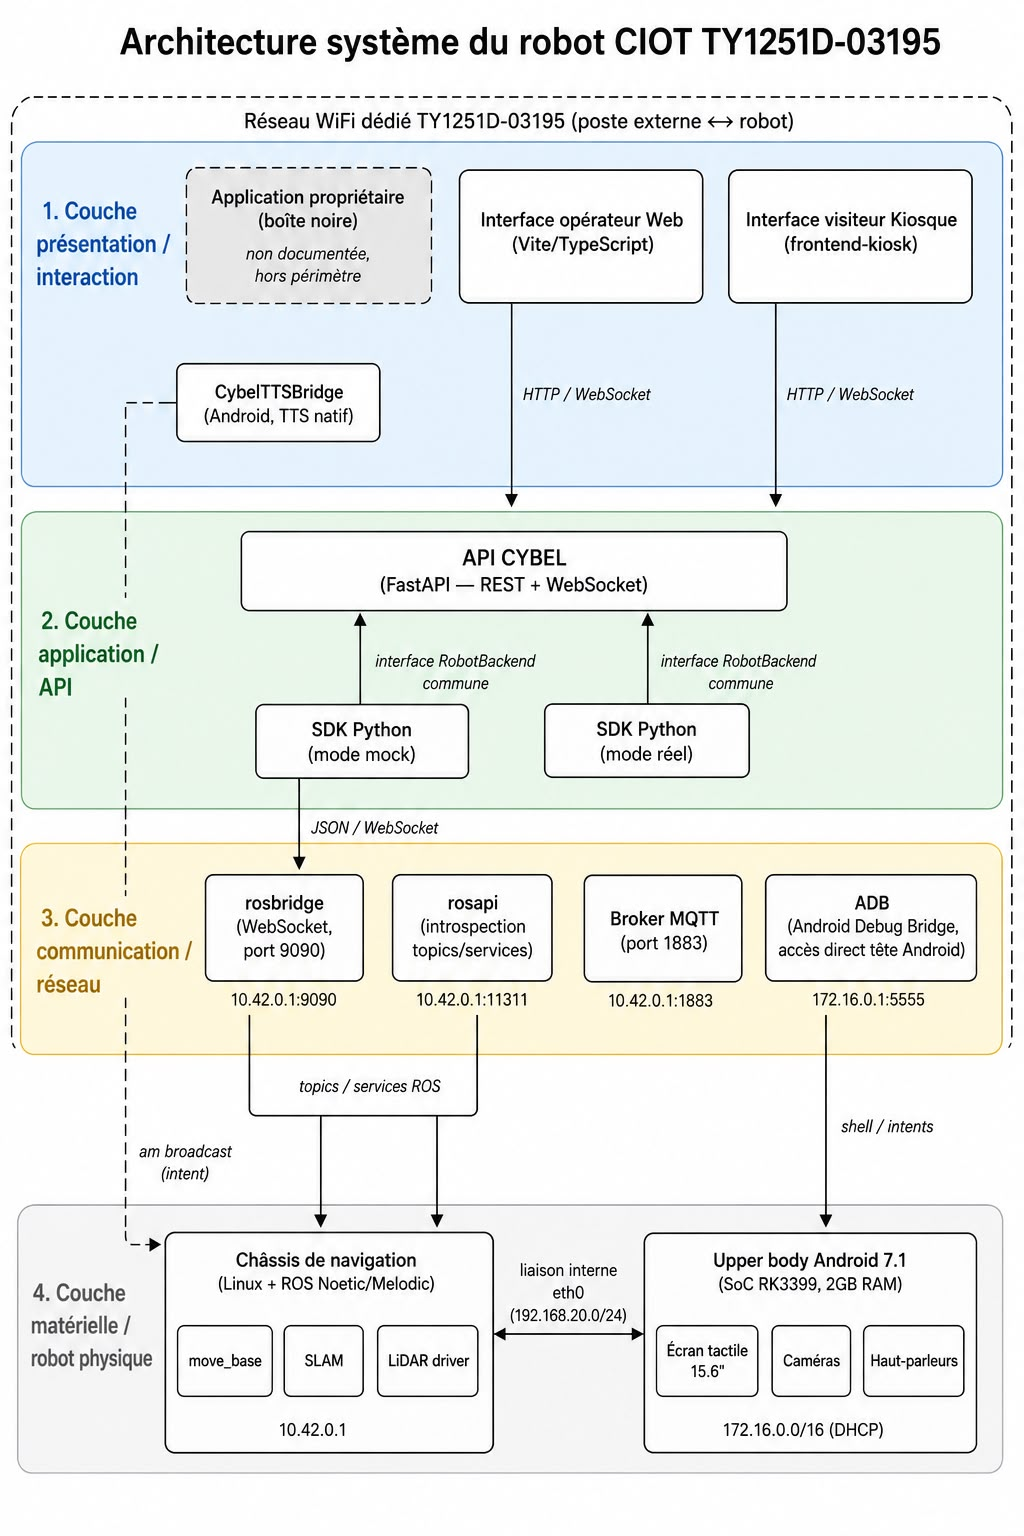
\includegraphics[width=0.7\textwidth]{diagramme/architecture_globale.jpeg}
    \captionof{figure}{Architecture système globale du robot CIOT TY1251D-03195}
    \label{fig:archi_robot}
\end{center}

\paragraph{Positionnement du système CYBEL dans l'architecture.}
Le système CYBEL s'insère principalement dans les couches supérieures de
l'architecture, en remplaçant et en étendant les capacités de l'application
propriétaire. Il s'appuie sur la couche applicative (API FastAPI et SDK
Python) pour structurer la logique de commande, sur la couche réseau
(rosbridge, MQTT) pour l'interaction avec le robot, et sur les couches
matérielles sous-jacentes pour l'exécution des actions physiques. Cette
approche permet de découpler totalement l'interface utilisateur du système
robotique, tout en garantissant une compatibilité avec l'infrastructure
existante.

L'architecture globale du système met ainsi en évidence une organisation en
couches clairement séparées, allant de l'interface utilisateur jusqu'au
matériel robotique. Cette structuration constitue le fondement de la
solution CYBEL, qui s'inscrit comme une couche logicielle intermédiaire
visant à unifier, simplifier et étendre l'accès aux fonctionnalités du robot
CIOT TY1251D-03195.

\subsubsection*{Cadre et déroulement du stage}

L'établissement disposant de ce robot souhaite l'utiliser pour des scénarios
d'accueil et de démonstration personnalisés : annonces vocales spécifiques,
déplacements vers des points définis par l'utilisateur, supervision à
distance. Le projet est encadré par HESTIM Engineering \& Business School et
s'adresse à des étudiants du cycle ingénieur (dont la
1\textsuperscript{re} année). Il est prévu sur une durée de trois à quatre mois, structuré en
quatre phases : (1) compréhension de l'architecture et établissement de la
connectivité réseau, (2) exploration et analyse du protocole de
communication interne, (3) développement de l'interface de commande et des
modules d'interaction, et (4) intégration, tests et validation finale.

\subsubsection*{Limites de la solution existante}

L'application propriétaire installée sur l'\textit{upper body} ne permet pas
le type de personnalisation recherché : elle constitue une boîte noire, sans
documentation, sans API exposée et sans code source disponible. Le
constructeur ne fournit par ailleurs aucune documentation technique sur les
protocoles de communication internes, ce qui interdit toute extension ou
adaptation directe de la solution d'origine.

\subsection{Problématique}

La problématique centrale du projet peut être formulée ainsi :

\begin{center}
\fbox{
    \parbox{0.9\textwidth}{
        \textit{Comment concevoir une plateforme de commande et d'interaction
        tierce, fonctionnellement équivalente ou supérieure à l'application
        propriétaire d'un robot de service Android, en l'absence de toute
        documentation officielle sur ses interfaces de communication internes ?}
    }
}
\end{center}

\medskip
Cette problématique se décline en plusieurs sous-questions :

\begin{itemize}
    \item Quels sont les \textbf{points d'accès réseau} (adresses IP, ports,
    protocoles) exposés par le robot, et lesquels sont effectivement exploitables
    sans authentification propriétaire ?
    \item Quel est le \textbf{format des messages} échangés entre l'interface
    Android et le système de navigation (ROS), et peut-il être reconstruit par
    observation et introspection plutôt que par décompilation de l'application ?
    \item Comment \textbf{distinguer une commande effectivement traitée par le
    robot d'une commande silencieusement ignorée}, dans un système où le protocole
    de transport (\texttt{rosbridge}) ne renvoie pas systématiquement d'erreur
    explicite ?
    \item Comment concevoir une architecture logicielle qui reste
    \textbf{utilisable et testable sans accès permanent au robot physique}
    (contraintes de disponibilité du matériel), tout en restant fidèle au
    comportement réel une fois connectée ?
    \item Dans quelle mesure les fonctionnalités d'\textbf{interaction homme-robot}
    (synthèse vocale, reconnaissance vocale, retour visuel) peuvent-elles être
    reconstruites lorsque le canal correspondant n'est pas exposé par le système
    de navigation (ROS) et nécessite un accès direct au sous-système Android ?
\end{itemize}

\subsection{Objectifs du projet}

\subsubsection{Objectif général}

Concevoir et développer une \textbf{plateforme web indépendante} de commande,
de supervision et d'interaction pour le robot CIOT TY1251D-03195, sans
dépendre de l'application Android propriétaire, en documentant de façon
rigoureuse le \textbf{protocole de communication} reconstruit (endpoints,
topics, services, formats de messages) afin que ce travail puisse être
réutilisé ou étendu.

\subsubsection{Objectifs spécifiques}

\begin{enumerate}
    \item \textbf{Établir la connectivité} avec le robot (réseau WiFi dédié,
    identification des hôtes et ports actifs).
    \item \textbf{Identifier les points de communication} exposés : WebSocket
    \texttt{rosbridge} (port 9090), broker \texttt{MQTT} (port 1883), services
    FTP/SSH, interfaces web internes (\texttt{:8082}, \texttt{:8088}).
    \item \textbf{Capturer et analyser le trafic réseau} afin de reconstituer
    les topics et services ROS pertinents (mouvement, navigation, télémétrie,
    capteurs).
    \item \textbf{Décoder et reconstruire les commandes de contrôle} du
    mouvement et de la navigation (vitesse, position cible, annulation de
    trajectoire).
    \item \textbf{Développer une interface de commande web} (backend FastAPI
    + frontend TypeScript) permettant la supervision temps réel et l'envoi de
    commandes.
    \item \textbf{Implémenter des fonctionnalités d'interaction homme-robot de
    base} : navigation par sélection de points ou clic sur carte, retour vocal
    (TTS) et commande vocale opérateur.
    \item \textbf{Mettre en place un mode de simulation (« mock »)} permettant
    de développer et tester l'interface sans dépendre de la disponibilité
    physique du robot.
    \item \textbf{Intégrer l'ensemble des composants} (SDK Python, API, interface
    web) dans un système cohérent et démontrable.
\end{enumerate}

\subsection{Cahier des charges}

\subsubsection{Périmètre du projet}

Le tableau~\ref{tab:perimetre_projet} délimite les activités prises en
charge par le projet de celles volontairement laissées hors périmètre.

\begin{center}
\begin{tabular}{|p{0.46\textwidth}|p{0.46\textwidth}|}
\hline
\textbf{Inclus dans le périmètre} & \textbf{Exclu du périmètre} \\
\hline
Identification et documentation des canaux de communication du robot
(\texttt{rosbridge}, MQTT, services réseau) &
Modification du firmware ou du logiciel embarqué du robot \\
\hline
Développement d'un SDK Python d'accès au robot (mode simulé et mode réel) &
Développement d'une application Android de remplacement (optionnel, non engagé) \\
\hline
Développement d'une API de commande/supervision (FastAPI) &
Décompilation ou rétro-ingénierie de l'application Android propriétaire \\
\hline
Développement d'une interface web opérateur (Vite/TypeScript) &
Déploiement en production / hébergement distant \\
\hline
Fonctionnalités de navigation (point nommé, clic sur carte, téléopération) &
Comportements autonomes avancés (planification de mission, multi-robot) \\
\hline
Interaction de base : synthèse vocale (TTS) et commande vocale opérateur &
Vision par caméra, reconnaissance faciale, chatbot (extensions optionnelles) \\
\hline
Documentation technique et rapport de stage &
Formation des utilisateurs finaux / exploitation au long cours \\
\hline
\end{tabular}
\captionof{table}{Périmètre du projet : éléments inclus et exclus}
\label{tab:perimetre_projet}
\end{center}

\subsubsection{Acteurs du système}

Le tableau~\ref{tab:acteurs_systeme} identifie les principaux acteurs
impliqués dans le projet ainsi que leur rôle respectif.

\begin{center}
\begin{tabular}{|p{0.35\textwidth}|p{0.57\textwidth}|}
\hline
\textbf{Acteur} & \textbf{Rôle} \\
\hline
Étudiant(e) stagiaire — plateforme CYBEL (C. Lusamote Kimfuta) &
Rétro-ingénierie, SDK, backend, interfaces web, Android, déploiement Termux,
documentation technique, contenu du présent rapport \\
\hline
Étudiant(e) stagiaire — chatbot (G. Khalifi) &
Développement d'un module chatbot sur la branche
\texttt{chatbot-cybel-projet-2026} du dépôt GitHub (hors périmètre CYBEL) \\
\hline
Encadrante pédagogique (Mme MESKINI, HESTIM) &
Suivi pédagogique, validation académique du rapport \\
\hline
Encadrant en entreprise (M. Tula, HESTIM) &
Suivi technique du robot, validation des objectifs sur le terrain \\
\hline
Établissement d'accueil &
Mise à disposition du robot et de l'environnement de travail \\
\hline
Opérateur final &
Supervision et pilotage du robot via la plateforme CYBEL \\
\hline
Robot CIOT TY1251D-03195 &
Système cible — serveur de télémétrie et de commandes via \texttt{rosbridge}/MQTT \\
\hline
\end{tabular}
\captionof{table}{Acteurs du système et leurs rôles}
\label{tab:acteurs_systeme}
\end{center}

\subsubsection{Besoins fonctionnels}

Le tableau~\ref{tab:besoins_fonctionnels} liste les exigences fonctionnelles
du système, accompagnées de leur niveau de priorité.

\begin{center}
\begin{tabular}{|p{0.10\textwidth}|p{0.67\textwidth}|p{0.13\textwidth}|}
\hline
\textbf{Réf.} & \textbf{Exigence} & \textbf{Priorité} \\
\hline
EF-01 & Superviser en temps réel l'état du robot (batterie, position, statut,
mode de navigation) & Essentielle \\
\hline
EF-02 & Afficher la carte SLAM, le LiDAR et les personnes détectées & Essentielle \\
\hline
EF-03 & Naviguer vers un point nommé prédéfini & Essentielle \\
\hline
EF-04 & Naviguer vers une coordonnée choisie par clic sur la carte, avec prise
en compte des obstacles & Essentielle \\
\hline
EF-05 & Téléopérer manuellement le robot (vitesse linéaire/angulaire) avec arrêt
d'urgence & Essentielle \\
\hline
EF-06 & Déclencher une annonce vocale sur le robot (TTS) & Souhaitable \\
\hline
EF-07 & Donner des commandes vocales à l'opérateur via le micro du navigateur &
Souhaitable \\
\hline
EF-08 & Configurer les paramètres de fonctionnement (vitesse, mode de
déplacement) & Souhaitable \\
\hline
EF-09 & Fonctionner en mode simulation complet sans robot connecté & Essentielle \\
\hline
\end{tabular}
\captionof{table}{Besoins fonctionnels du système}
\label{tab:besoins_fonctionnels}
\end{center}

\subsubsection{Besoins non fonctionnels}

Le tableau~\ref{tab:besoins_non_fonctionnels} présente les exigences non
fonctionnelles, relatives notamment à la performance, à la robustesse et à
la séparation des responsabilités au sein de l'architecture.

\begin{center}
\begin{tabular}{|p{0.10\textwidth}|p{0.67\textwidth}|p{0.13\textwidth}|}
\hline
\textbf{Réf.} & \textbf{Exigence} & \textbf{Priorité} \\
\hline
ENF-01 & Latence d'affichage de la télémétrie de l'ordre de quelques centaines
de ms maximum & Essentielle \\
\hline
ENF-02 & Reconnexion automatique au robot après perte de connexion réseau &
Essentielle \\
\hline
ENF-03 & Séparation stricte entre couche d'accès robot (SDK), API et présentation
& Essentielle \\
\hline
ENF-04 & Toute commande de mouvement/navigation doit être annulable à tout moment
& Essentielle \\
\hline
ENF-05 & Aucune action exploratoire ne doit perturber le fonctionnement normal
du robot & Essentielle \\
\hline
\end{tabular}
\captionof{table}{Besoins non fonctionnels du système}
\label{tab:besoins_non_fonctionnels}
\end{center}

\subsubsection{Contraintes du projet}

\begin{itemize}
    \item \textbf{Contraintes techniques} : absence de documentation officielle
    du protocole ; dépendance à un réseau WiFi dédié et potentiellement instable
    (latence variable, de 7 à 1654 ms observés) ; version Android embarquée
    obsolète (7.1) limitant les outils de débogage disponibles.

    \item \textbf{Contraintes matérielles} : un seul exemplaire de robot
    disponible, partagé avec d'autres usages de l'établissement — disponibilité
    limitée pour les tests.

    \item \textbf{Contraintes organisationnelles} : durée de stage limitée à
    trois à quatre mois ; deux stagiaires avec des périmètres distincts
    (plateforme CYBEL et chatbot) ; encadrement pédagogique et terrain
    périodique.

    \item \textbf{Contraintes de sécurité et d'éthique} : les canaux
    \texttt{rosbridge} et MQTT du robot étant accessibles sans authentification,
    toute manipulation doit respecter un principe de \textbf{précaution}
    (vérification en mode simulation avant toute commande réelle, mécanisme
    d'annulation disponible) ; les tentatives d'accès aux comptes système (SSH/FTP)
    doivent rester mesurées pour ne pas provoquer de blocage.

    \item \textbf{Contraintes de propriété intellectuelle} : aucune décompilation
    du logiciel propriétaire n'est entreprise ; seule l'observation du trafic
    réseau et l'introspection des interfaces standard (ROS, MQTT) sont utilisées.
\end{itemize}

\subsubsection{Livrables attendus}

Conformément au sujet de stage, les livrables attendus en fin de projet sont :

\begin{enumerate}
    \item Une \textbf{interface de communication fonctionnelle} avec le robot
    (SDK + client \texttt{rosbridge}/MQTT).
    \item Un \textbf{système de contrôle du mouvement} opérationnel
    (téléopération + navigation).
    \item Une \textbf{interface utilisateur} web opérateur.
    \item Un \textbf{module d'interaction de base} (tactile et/ou vocal).
    \item Un \textbf{rapport technique} incluant l'architecture du système et
    l'analyse du protocole.
\end{enumerate}

\subsubsection{Critères de réception et de validation}

Le tableau~\ref{tab:criteres_validation} précise, pour chaque critère
d'acceptation, la modalité de vérification associée.

\begin{center}
\begin{tabular}{|p{0.40\textwidth}|p{0.52\textwidth}|}
\hline
\textbf{Critère} & \textbf{Modalité de vérification} \\
\hline
Connexion au robot établie de façon reproductible &
Connexion \texttt{rosbridge} réussie depuis le réseau WiFi du robot, vérifiable
via \texttt{/rosapi/topics} \\
\hline
Télémétrie affichée en temps réel &
Observation du tableau de bord (position, batterie, statut) à jour \\
\hline
Navigation vers un point ou une coordonnée &
Envoi d'une commande de navigation suivie d'un changement d'état
(\texttt{/navi\_status}) cohérent \\
\hline
Téléopération et arrêt d'urgence &
Test en mode simulation puis, si possible, sur robot réel à vitesse réduite \\
\hline
Fonctionnement en mode simulation &
Lancement avec \texttt{ROBOT\_MOCK=true}, toutes les fonctionnalités principales
accessibles \\
\hline
Interaction vocale &
TTS robot \textbf{ou} solution de repli (voix opérateur via navigateur)
fonctionnelle \\
\hline
Documentation &
Présence et cohérence de \texttt{README.md}, \texttt{docs/INTERFACE.md} et du
présent rapport \\
\hline
\end{tabular}
\captionof{table}{Critères de réception et de validation}
\label{tab:criteres_validation}
\end{center}

\subsection{Solution proposée}

Face à ce besoin, la solution retenue consiste en une plateforme logicielle
indépendante, structurée autour d'une couche d'accès au robot (SDK Python
interchangeable mock/réel), d'une API de commande et de supervision, et
d'interfaces utilisateur web dédiées à l'opérateur et au visiteur. L'analyse
fonctionnelle détaillée, l'architecture logicielle complète et les
diagrammes de conception associés sont présentés au Chapitre 4 (\textit{Analyse
et conception du système}).

\subsection{Conclusion}

Ce chapitre a permis de poser le cadre du projet CYBEL : l'architecture du
robot CIOT TY1251D-03195 et les limites de sa solution propriétaire, la
problématique de rétro-ingénierie et de conception qui en découle, les
objectifs poursuivis, ainsi qu'un cahier des charges détaillant acteurs,
besoins, contraintes, livrables et critères de validation. Le chapitre
suivant situe ce travail par rapport à l'état de l'art en robotique de
service, architectures logicielles robotiques et interaction homme-robot.
\newpage
\section{ État de l'art}
\label{chap:etat_art}

Ce chapitre situe le projet CYBEL par rapport aux travaux et solutions
existants. Il présente les fondements théoriques de la robotique de service
ainsi que les solutions logicielles et matérielles comparables, afin de
mettre en évidence les limites des approches actuelles et de justifier les
choix architecturaux retenus.

\subsection{Fondements théoriques}
\label{subsec:fondements_theoriques}

La conception de la plateforme s'appuie sur plusieurs corpus de référence :

\begin{itemize}
    \item \textbf{Architecture logicielle robotique} : le modèle ROS
    (topics, services, actions) proposé par Quigley et al. constitue le
    paradigme de communication analysé dans ce projet.

    \item \textbf{Navigation autonome} : les concepts de cartes
    d'occupation et de planification (costmaps, DWA) décrits dans
    \textit{Probabilistic Robotics} (Thrun, Burgard \& Fox, 2005)
    servent de base à l'interprétation du module \texttt{move\_base}.

    \item \textbf{Protocole rosbridge} : le standard JSON de communication
    ROS (subscribe, publish, call\_service) est utilisé comme référence pour
    la reconstruction des échanges observés.

    \item \textbf{Interaction homme-robot (HRI)} : les principes de
    supervision en temps réel et de sécurité opérationnelle (priorité à
    l'arrêt d'urgence) guident la conception de l'interface CYBEL.

    \item \textbf{Sécurité IoT} : les recommandations de l'OWASP IoT Top 10
    permettent d'analyser les risques liés aux canaux non authentifiés
    observés sur le système.
\end{itemize}

\subsection{État des solutions existantes}
\label{subsec:solutions_existantes}

Les solutions suivantes représentent les principales approches disponibles
dans l'écosystème robotique et du robot étudié.

\begin{table}[h!]
\centering
\begin{tabular}{|p{0.28\textwidth}|p{0.38\textwidth}|p{0.24\textwidth}|}
\hline
\textbf{Solution} & \textbf{Description} & \textbf{Accessibilité} \\
\hline
Application propriétaire (upper body Android) &
Interface tactile constructeur pour accueil et navigation &
Fermée, sans API ni documentation \\
\hline
Interface web embarquée (\texttt{:8082}) &
Outil de gestion des cartes SLAM &
Accessible localement, non documenté \\
\hline
Interface de debug (\texttt{:8088}) &
Interface interne de diagnostic &
Non documentée, usage inconnu \\
\hline
rosbridge / RViz / Foxglove &
Outils ROS de visualisation et contrôle &
Open-source mais génériques \\
\hline
SDK robots commerciaux (Temi, Pepper, etc.) &
SDK propriétaires pour robots de service &
Documentés mais verrouillés \\
\hline
\end{tabular}
\caption{Panorama des solutions existantes comparables}
\label{tab:solutions_existantes}
\end{table}

\subsection{Analyse comparative}
\label{subsec:benchmark}

\begin{table}[h!]
\centering
\begin{tabular}{|p{0.28\textwidth}|p{0.20\textwidth}|p{0.20\textwidth}|p{0.20\textwidth}|}
\hline
\textbf{Critère} &
\textbf{App. propriétaire} &
\textbf{RViz / Foxglove} &
\textbf{CYBEL} \\
\hline
Documentation &
Aucune &
Open-source &
Documenté (rapport + code) \\
\hline
Accès distant web &
Non &
Partiel &
Oui \\
\hline
Personnalisation scénarios &
Non &
Non &
Oui \\
\hline
Mode simulation &
Non &
Partiel &
Oui (mock) \\
\hline
Navigation interactive &
Oui &
Oui &
Oui + logique métier \\
\hline
Interaction vocale &
Oui &
Non &
Partiel / évolutif \\
\hline
\end{tabular}
\caption{Benchmark comparatif des solutions}
\label{tab:benchmark_cybel}
\end{table}

\subsection{Limites des solutions existantes}
\label{subsec:limites}

Les solutions étudiées présentent plusieurs limites majeures :

\begin{itemize}
    \item Absence d'extensibilité des systèmes propriétaires
    \item Outils ROS de trop bas niveau pour des usages métier
    \item Aucune solution ne propose de mode déconnecté du robot
    \item Documentation constructeur insuffisante nécessitant rétro-ingénierie
\end{itemize}

\subsection{Synthèse}
\label{subsec:synthese_etat_art}

L'analyse met en évidence un manque de solutions adaptées à un usage
orienté \textbf{scénarios d'accueil personnalisés} et \textbf{supervision
haut niveau}. Ces limites justifient le développement de la plateforme
CYBEL, détaillée dans le chapitre suivant.

\subsection{Conclusion}
\label{subsec:conclusion_etat_art}

Ce chapitre a permis de situer le projet CYBEL par rapport aux fondements
théoriques de la robotique de service architecture ROS, navigation
autonome, protocole \texttt{rosbridge}, interaction homme-robot et sécurité
des objets connectés ainsi qu'aux solutions existantes, qu'elles soient
propriétaires (application Android constructeur) ou génériques (rosbridge,
RViz, Foxglove, SDK de robots commerciaux). L'analyse comparative a montré
qu'aucune de ces solutions ne répond pleinement aux besoins identifiés au
Chapitre 2 : extensibilité, logique métier orientée accueil, supervision
de haut niveau et mode de développement déconnecté du robot physique. Ces
limites confirment la pertinence du projet CYBEL et orientent directement
les choix de conception présentés au Chapitre 4, qui détaille l'analyse
fonctionnelle et l'architecture logicielle de la solution retenue.

%================================================
% PARTIE 2 : CONCEPTION ET DÉVELOPPEMENT
%================================================
\newpage
\section{Chapitre 4 : Analyse et conception du système}

Ce chapitre présente l'analyse fonctionnelle du système CYBEL ainsi que les
choix de conception retenus pour répondre au cahier des charges défini au
chapitre précédent. Il détaille successivement les acteurs et les besoins
identifiés, l'architecture générale et logicielle de la plateforme, les
diagrammes de conception (composants, cas d'utilisation, séquence) et le
modèle des flux de communication entre les différents sous-systèmes.

\subsection{Analyse fonctionnelle}

Après l'étude du besoin et l'analyse des solutions existantes, il est
nécessaire de définir précisément le fonctionnement du système à concevoir.
Cette phase d'analyse fonctionnelle permet d'identifier les acteurs
intervenant dans le système, les services qui leur sont proposés ainsi que
les interactions nécessaires à la réalisation des différentes
fonctionnalités.

Le projet CYBEL vise à fournir une plateforme de supervision, de commande
et d'interaction destinée au robot de service CIOT TY1251D-03195, déployé
au sein du FabLab de HESTIM. Cette plateforme doit permettre aux opérateurs
de piloter le robot, de suivre son état en temps réel et de gérer les
interactions avec les visiteurs, tout en assurant une communication fiable
avec les différents composants matériels et logiciels du système.

L'analyse fonctionnelle constitue ainsi une étape essentielle avant la
conception détaillée de l'architecture, puisqu'elle permet de traduire les
besoins exprimés dans le cahier des charges en fonctionnalités concrètes.

\subsubsection{Identification des acteurs}

L'étude des besoins a permis d'identifier trois acteurs principaux
intervenant dans le fonctionnement du système CYBEL.

\paragraph{L'opérateur.}
L'opérateur représente l'utilisateur chargé de l'administration et de la
supervision du robot. Il dispose d'une interface lui permettant de
consulter l'état du robot, de visualiser sa position sur la carte,
d'accéder aux informations de télémétrie, de lancer des scénarios de
navigation, de téléopérer le robot, de déclencher des annonces vocales et
de gérer les paramètres du système. Son rôle est central puisque c'est lui
qui assure le contrôle opérationnel du robot au sein du FabLab.

\paragraph{Le visiteur.}
Le visiteur interagit avec le robot à travers l'interface embarquée sur la
tablette Android. Cette interface lui permet notamment de découvrir les
différents espaces du FabLab, de sélectionner des points d'intérêt, de
consulter des informations de présentation et d'interagir avec le robot
lors des démonstrations. Le visiteur n'a pas accès aux fonctionnalités
d'administration ou de contrôle du système.

\paragraph{Le système CYBEL.}
Le système CYBEL constitue un acteur autonome chargé de coordonner les
différents composants logiciels. Il assure notamment la collecte des
données du robot, la diffusion de la télémétrie, la gestion des
communications, la reconnexion automatique en cas de perte de liaison, la
synchronisation des données entre les interfaces, ainsi que le
déclenchement des services associés à la navigation et à l'interaction.

\subsubsection{Besoins fonctionnels}

À partir de l'analyse du besoin, plusieurs fonctionnalités principales ont
été identifiées.

\paragraph{Supervision du robot.}
Le système doit permettre la consultation en temps réel du niveau de
batterie, de la position du robot, de son état de navigation, des données
LiDAR, des visiteurs détectés et des messages de diagnostic.

\paragraph{Navigation autonome.}
Le système doit permettre l'envoi du robot vers un point prédéfini, la
navigation vers une position sélectionnée sur la carte, l'annulation d'une
mission en cours, ainsi que le suivi de l'avancement de la navigation.

\paragraph{Téléopération.}
L'opérateur doit pouvoir contrôler manuellement les déplacements du robot
à travers une interface de commande ou un clavier virtuel.

\paragraph{Interaction Homme-Robot.}
Le système doit permettre le déclenchement d'annonces vocales, la
diffusion de messages d'accueil, l'utilisation de commandes vocales
opérateur, ainsi que l'affichage d'informations destinées aux visiteurs.

\paragraph{Configuration du système.}
L'opérateur doit pouvoir modifier certains paramètres de fonctionnement
tels que les vitesses de déplacement, les paramètres de navigation et les
réglages de communication.

\paragraph{Mode simulation.}
Le système doit être capable de fonctionner sans robot physique grâce à un
mode simulé permettant le développement et les tests des fonctionnalités.

\subsubsection{Besoins non fonctionnels}

Outre les fonctionnalités attendues, plusieurs contraintes de qualité ont
été retenues.

\paragraph{Performance.}
La plateforme doit assurer une mise à jour rapide des informations afin de
garantir une supervision efficace du robot.

\paragraph{Fiabilité.}
Le système doit maintenir la continuité des communications et assurer une
reconnexion automatique après une interruption réseau.

\paragraph{Maintenabilité.}
L'architecture doit favoriser l'évolution et la réutilisation du code
grâce à une séparation claire des responsabilités.

\paragraph{Sécurité.}
Les commandes critiques doivent pouvoir être annulées rapidement afin
d'éviter tout comportement indésirable du robot.

\paragraph{Ergonomie.}
Les interfaces doivent être simples d'utilisation et adaptées aussi bien
aux opérateurs qu'aux visiteurs.

\subsection{Architecture générale de CYBEL}

Afin de répondre aux besoins identifiés, une architecture modulaire a été
retenue. Celle-ci repose sur plusieurs composants indépendants
communiquant entre eux à travers des interfaces clairement définies.
L'objectif principal de cette architecture est de découpler les interfaces
utilisateur du système robotique afin de faciliter les tests, la
maintenance et l'évolution de la plateforme.

\begin{figure}[h!]
    \centering
    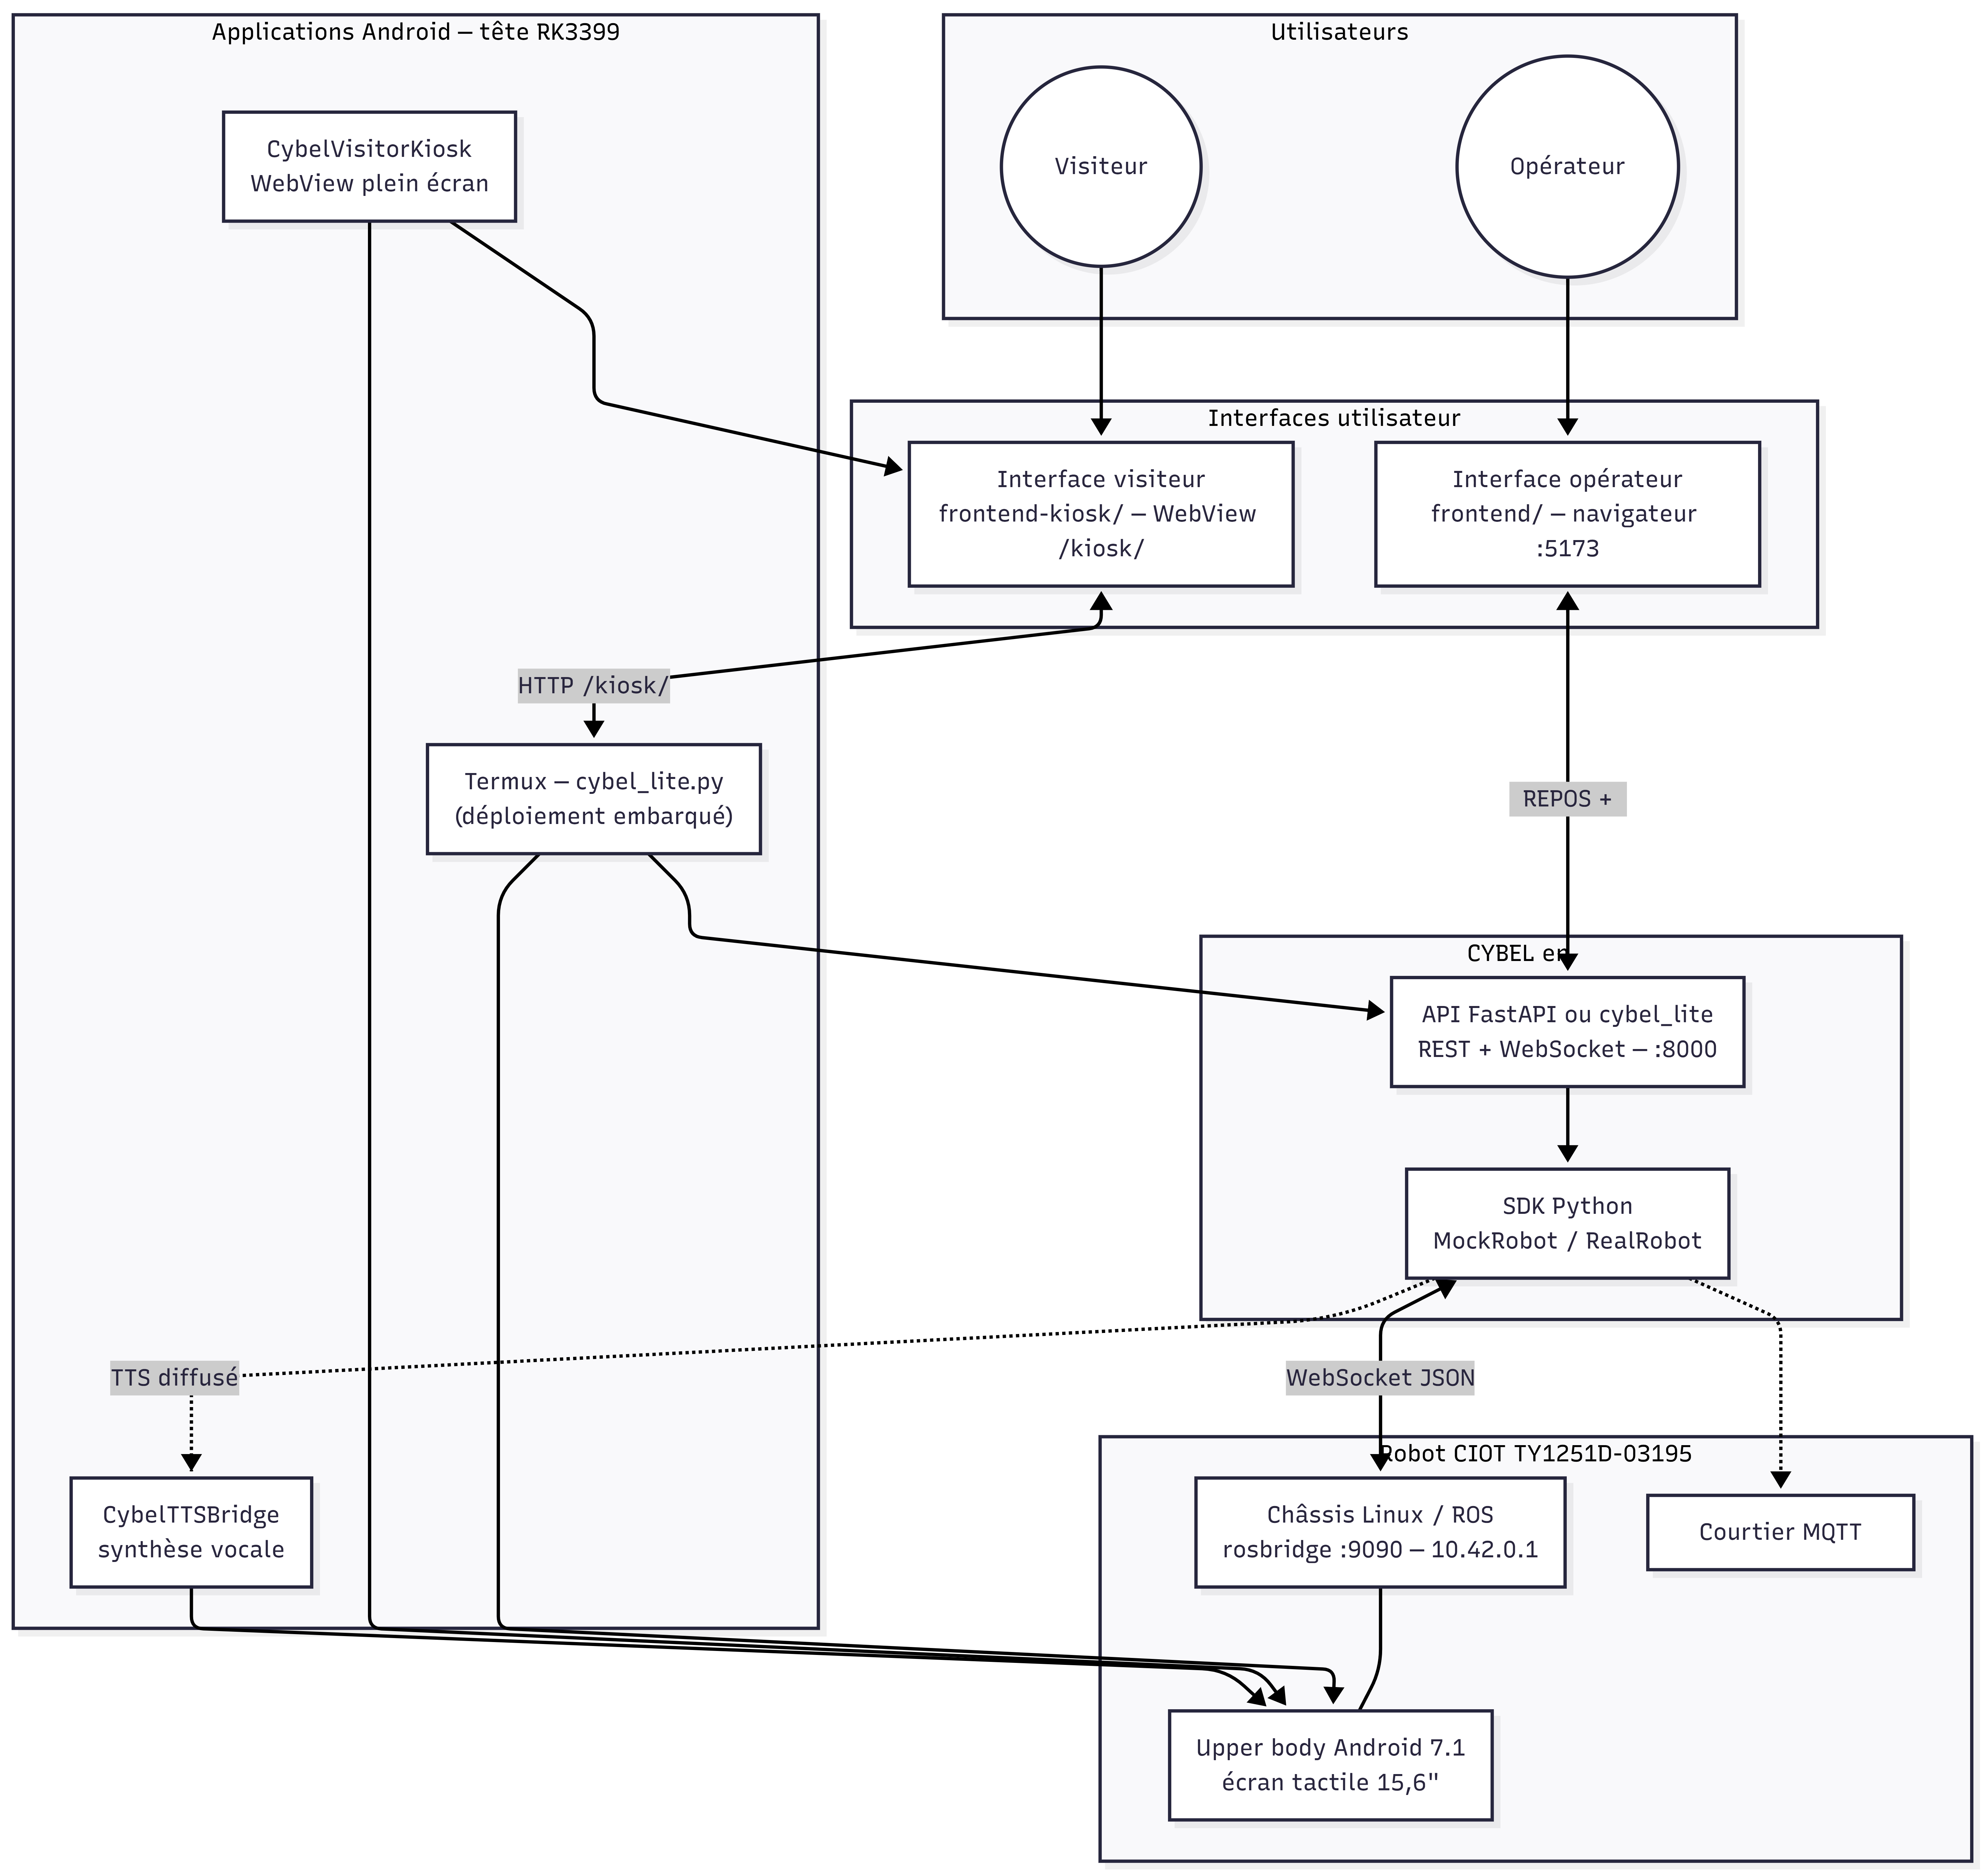
\includegraphics[width=0.9\textwidth]{diagramme/architecture_generale.png}
    \caption{Architecture générale du système CYBEL}
    \label{fig:archi_generale_cybel}
\end{figure}

Comme illustré en figure~\ref{fig:archi_generale_cybel}, l'architecture
globale du système s'articule autour de quatre ensembles principaux : le
robot CIOT TY1251D-03195, le backend CYBEL, les interfaces utilisateur et
les applications Android embarquées. Chaque composant joue un rôle
spécifique dans le fonctionnement global de la plateforme.

\subsection{Architecture logicielle}

L'architecture logicielle retenue suit une approche en couches permettant
de séparer les responsabilités fonctionnelles et techniques du système.
Elle est organisée autour de trois couches principales.

\subsubsection*{Couche d'accès au robot (SDK)}

Cette couche constitue l'abstraction du robot. Elle est responsable de la
communication avec ROSBridge, de la gestion du protocole reconstruit, de
l'accès aux données de télémétrie et de l'exécution des commandes. Deux
implémentations sont proposées : une implémentation réelle et une
implémentation simulée. Cette approche permet de développer et de tester
la plateforme sans dépendre de la disponibilité permanente du robot.

\subsubsection*{Couche API}

Cette couche repose sur FastAPI et constitue le point d'entrée principal
du système. Elle expose des services REST, des services WebSocket ainsi
que les mécanismes de gestion des événements. Elle joue également le rôle
d'intermédiaire entre les interfaces utilisateur et le SDK.

\subsubsection*{Couche présentation}

Cette couche regroupe l'interface opérateur, l'interface visiteur et les
applications Android complémentaires. Elle permet l'interaction entre les
utilisateurs et le système.

\begin{center}
    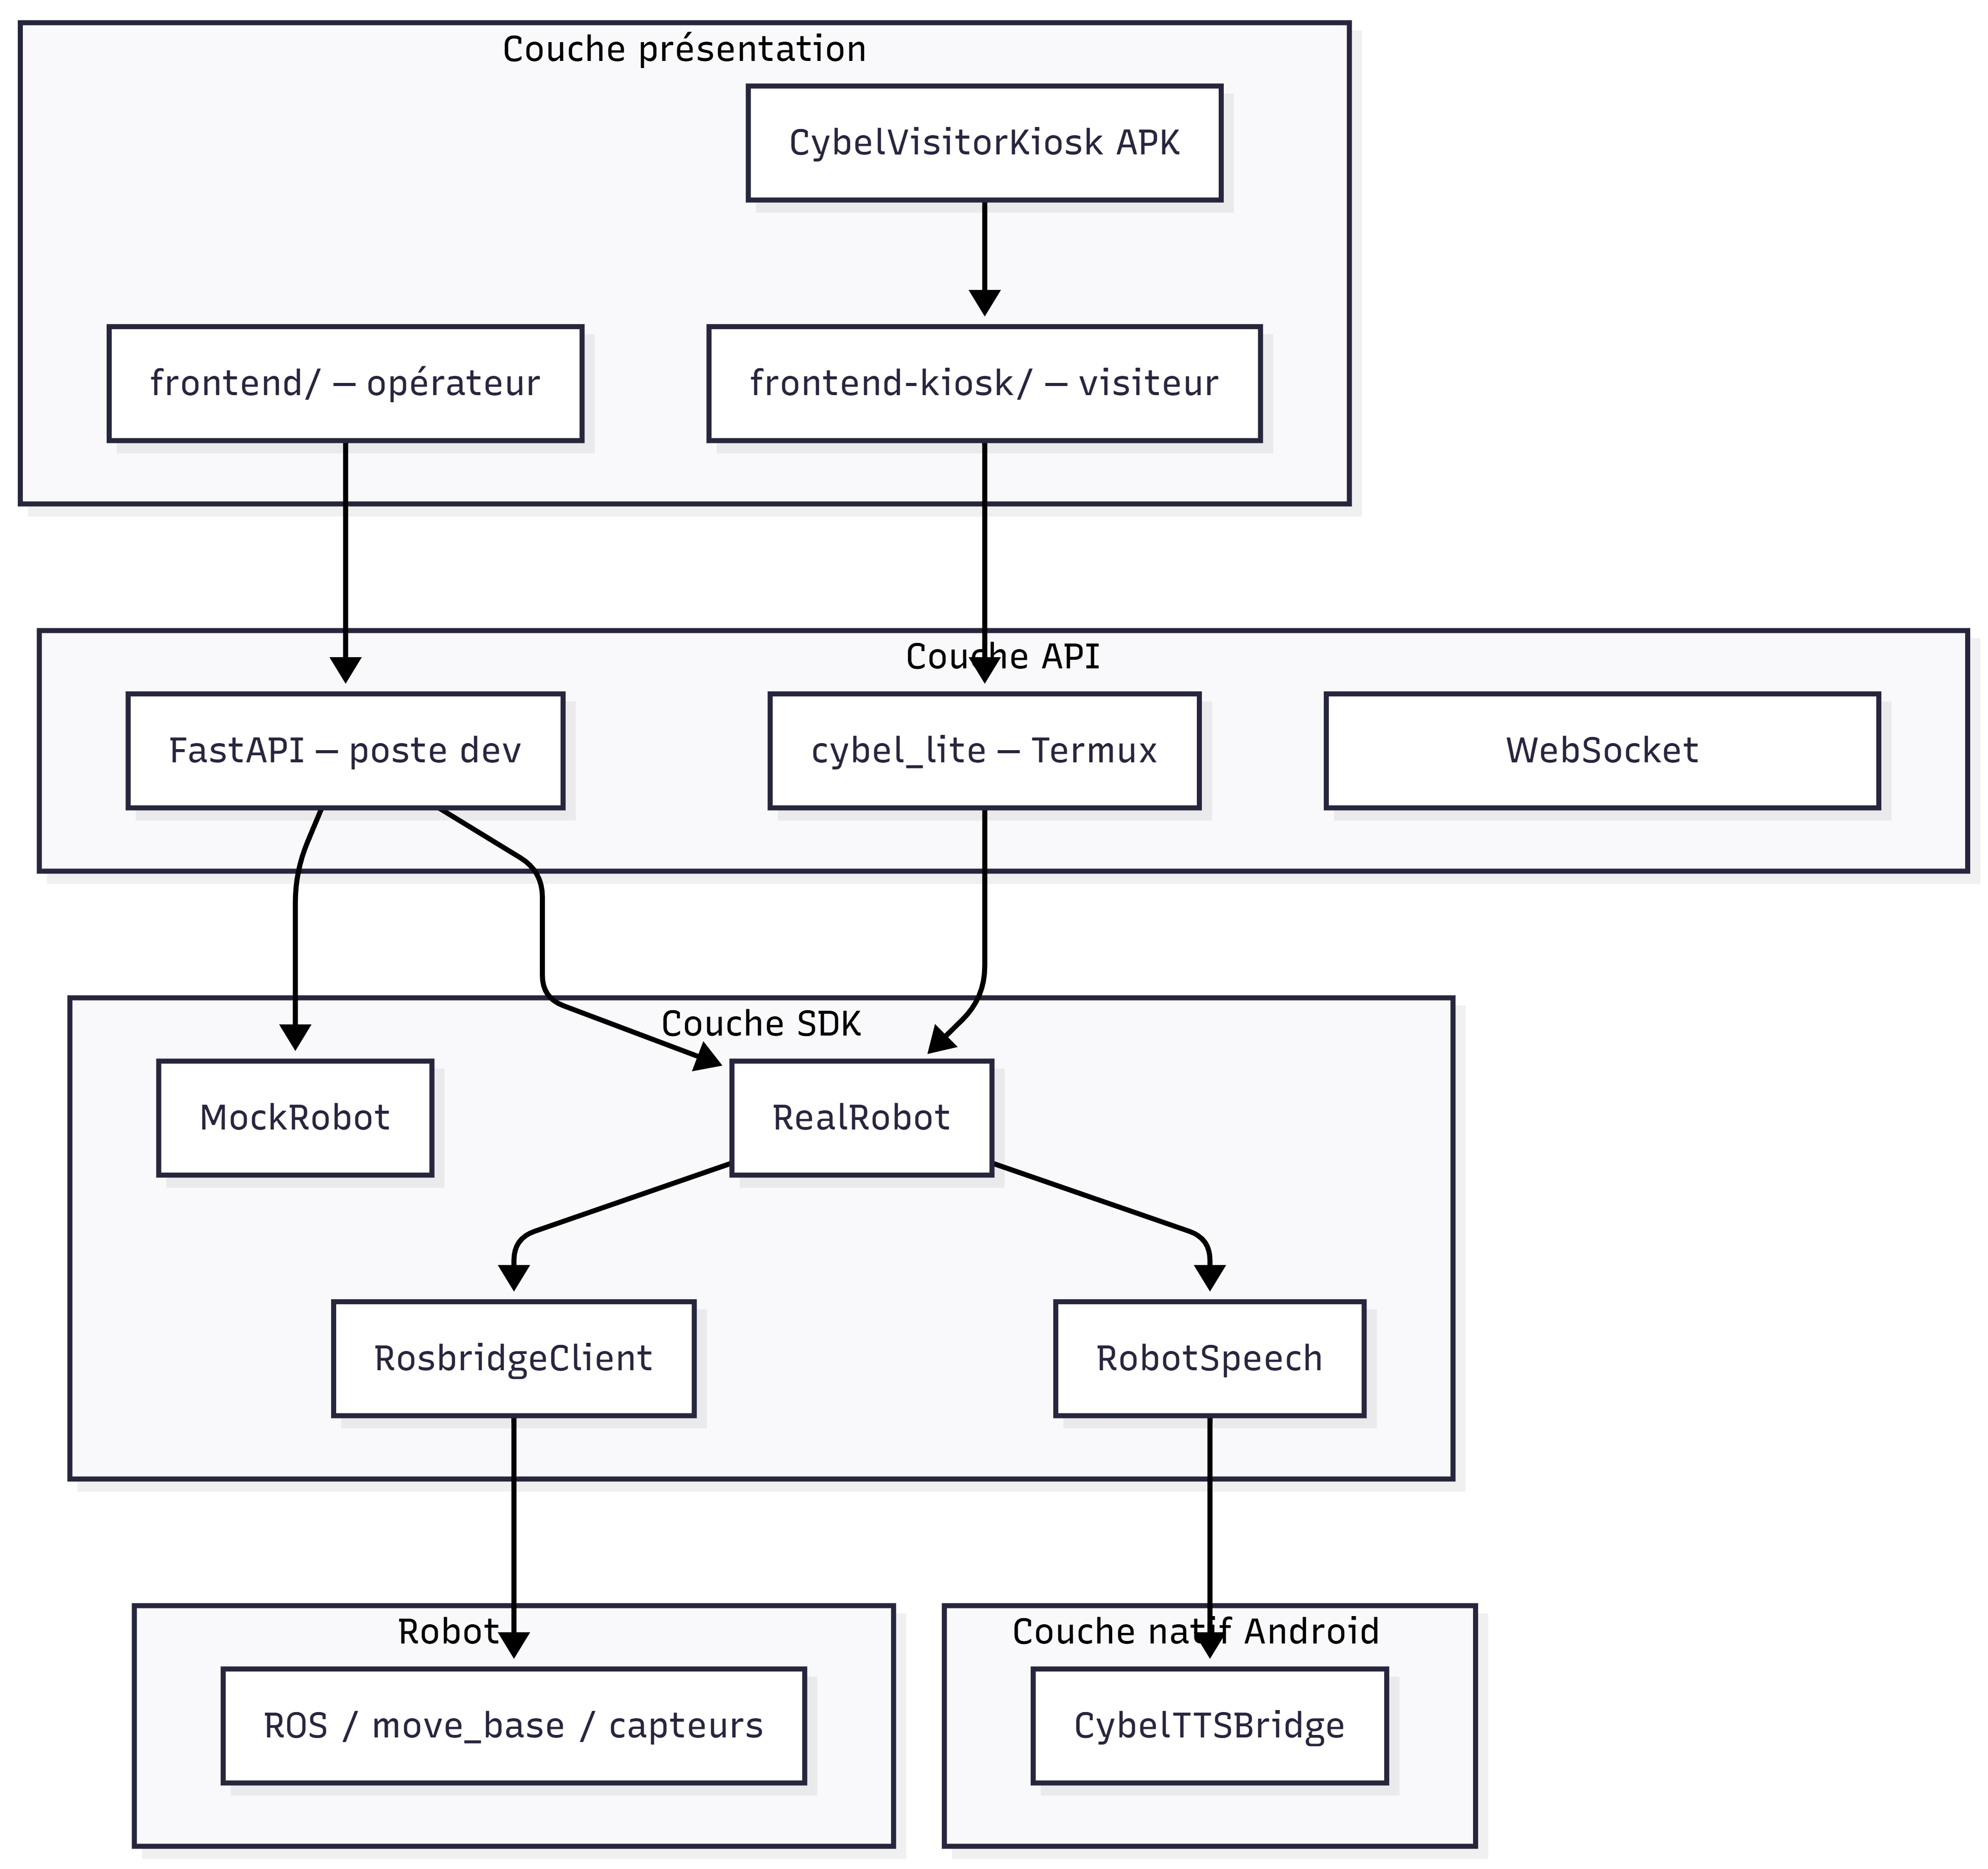
\includegraphics[width=0.8\textwidth]{diagramme/Architecture en couches-2026-06-20-163125.png}
    \captionof{figure}{Architecture en couches}
\end{center}

\subsection{Diagramme des composants}

Le diagramme des composants (figure~\ref{fig:diag_composants}) met en
évidence l'organisation des différents modules logiciels du système ainsi
que leurs dépendances. Il montre notamment les interfaces opérateur et
visiteur, le backend FastAPI, le SDK robot, ROSBridge, le système Android
embarqué ainsi que les modules TTS. Cette représentation permet de
visualiser clairement la répartition des responsabilités entre les
différents composants.

\begin{figure}[h!]
    \centering
    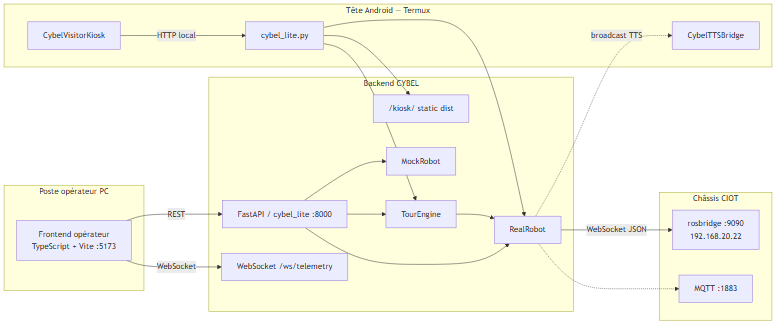
\includegraphics[width=0.85\textwidth]{diagramme/diagramme_composant.png}
    \caption{Diagramme de composants du système CYBEL}
    \label{fig:diag_composants}
\end{figure}

\subsection{Diagrammes de cas d'utilisation}

Les diagrammes de cas d'utilisation (figure~\ref{fig:diag_cas_usage})
permettent de représenter les interactions entre les acteurs identifiés et
les fonctionnalités proposées par le système. Ils mettent en évidence les
actions réalisées par l'opérateur, les interactions du visiteur, ainsi que
les traitements automatiques assurés par CYBEL.

\begin{figure}[h!]
    \centering
    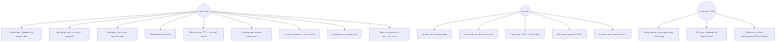
\includegraphics[width=0.9\textwidth]{diagramme/diagramme_cas_usage.png}
    \caption{Diagramme de cas d'utilisation du système CYBEL}
    \label{fig:diag_cas_usage}
\end{figure}

\subsection{Diagrammes de séquence}

Les diagrammes de séquence (figure~\ref{fig:diag_sequence}) permettent de
décrire l'enchaînement des échanges entre les différents composants du
système lors de l'exécution d'une fonctionnalité. Parmi les scénarios
étudiés figurent la navigation vers un point sélectionné, l'envoi d'une
commande de déplacement, le déclenchement d'une annonce vocale, ainsi que
la diffusion de la télémétrie vers l'interface opérateur. Ces diagrammes
facilitent la compréhension des mécanismes internes mis en \oe uvre lors
des communications entre le robot, le backend et les interfaces
utilisateur.

\begin{figure}[h!]
    \centering
    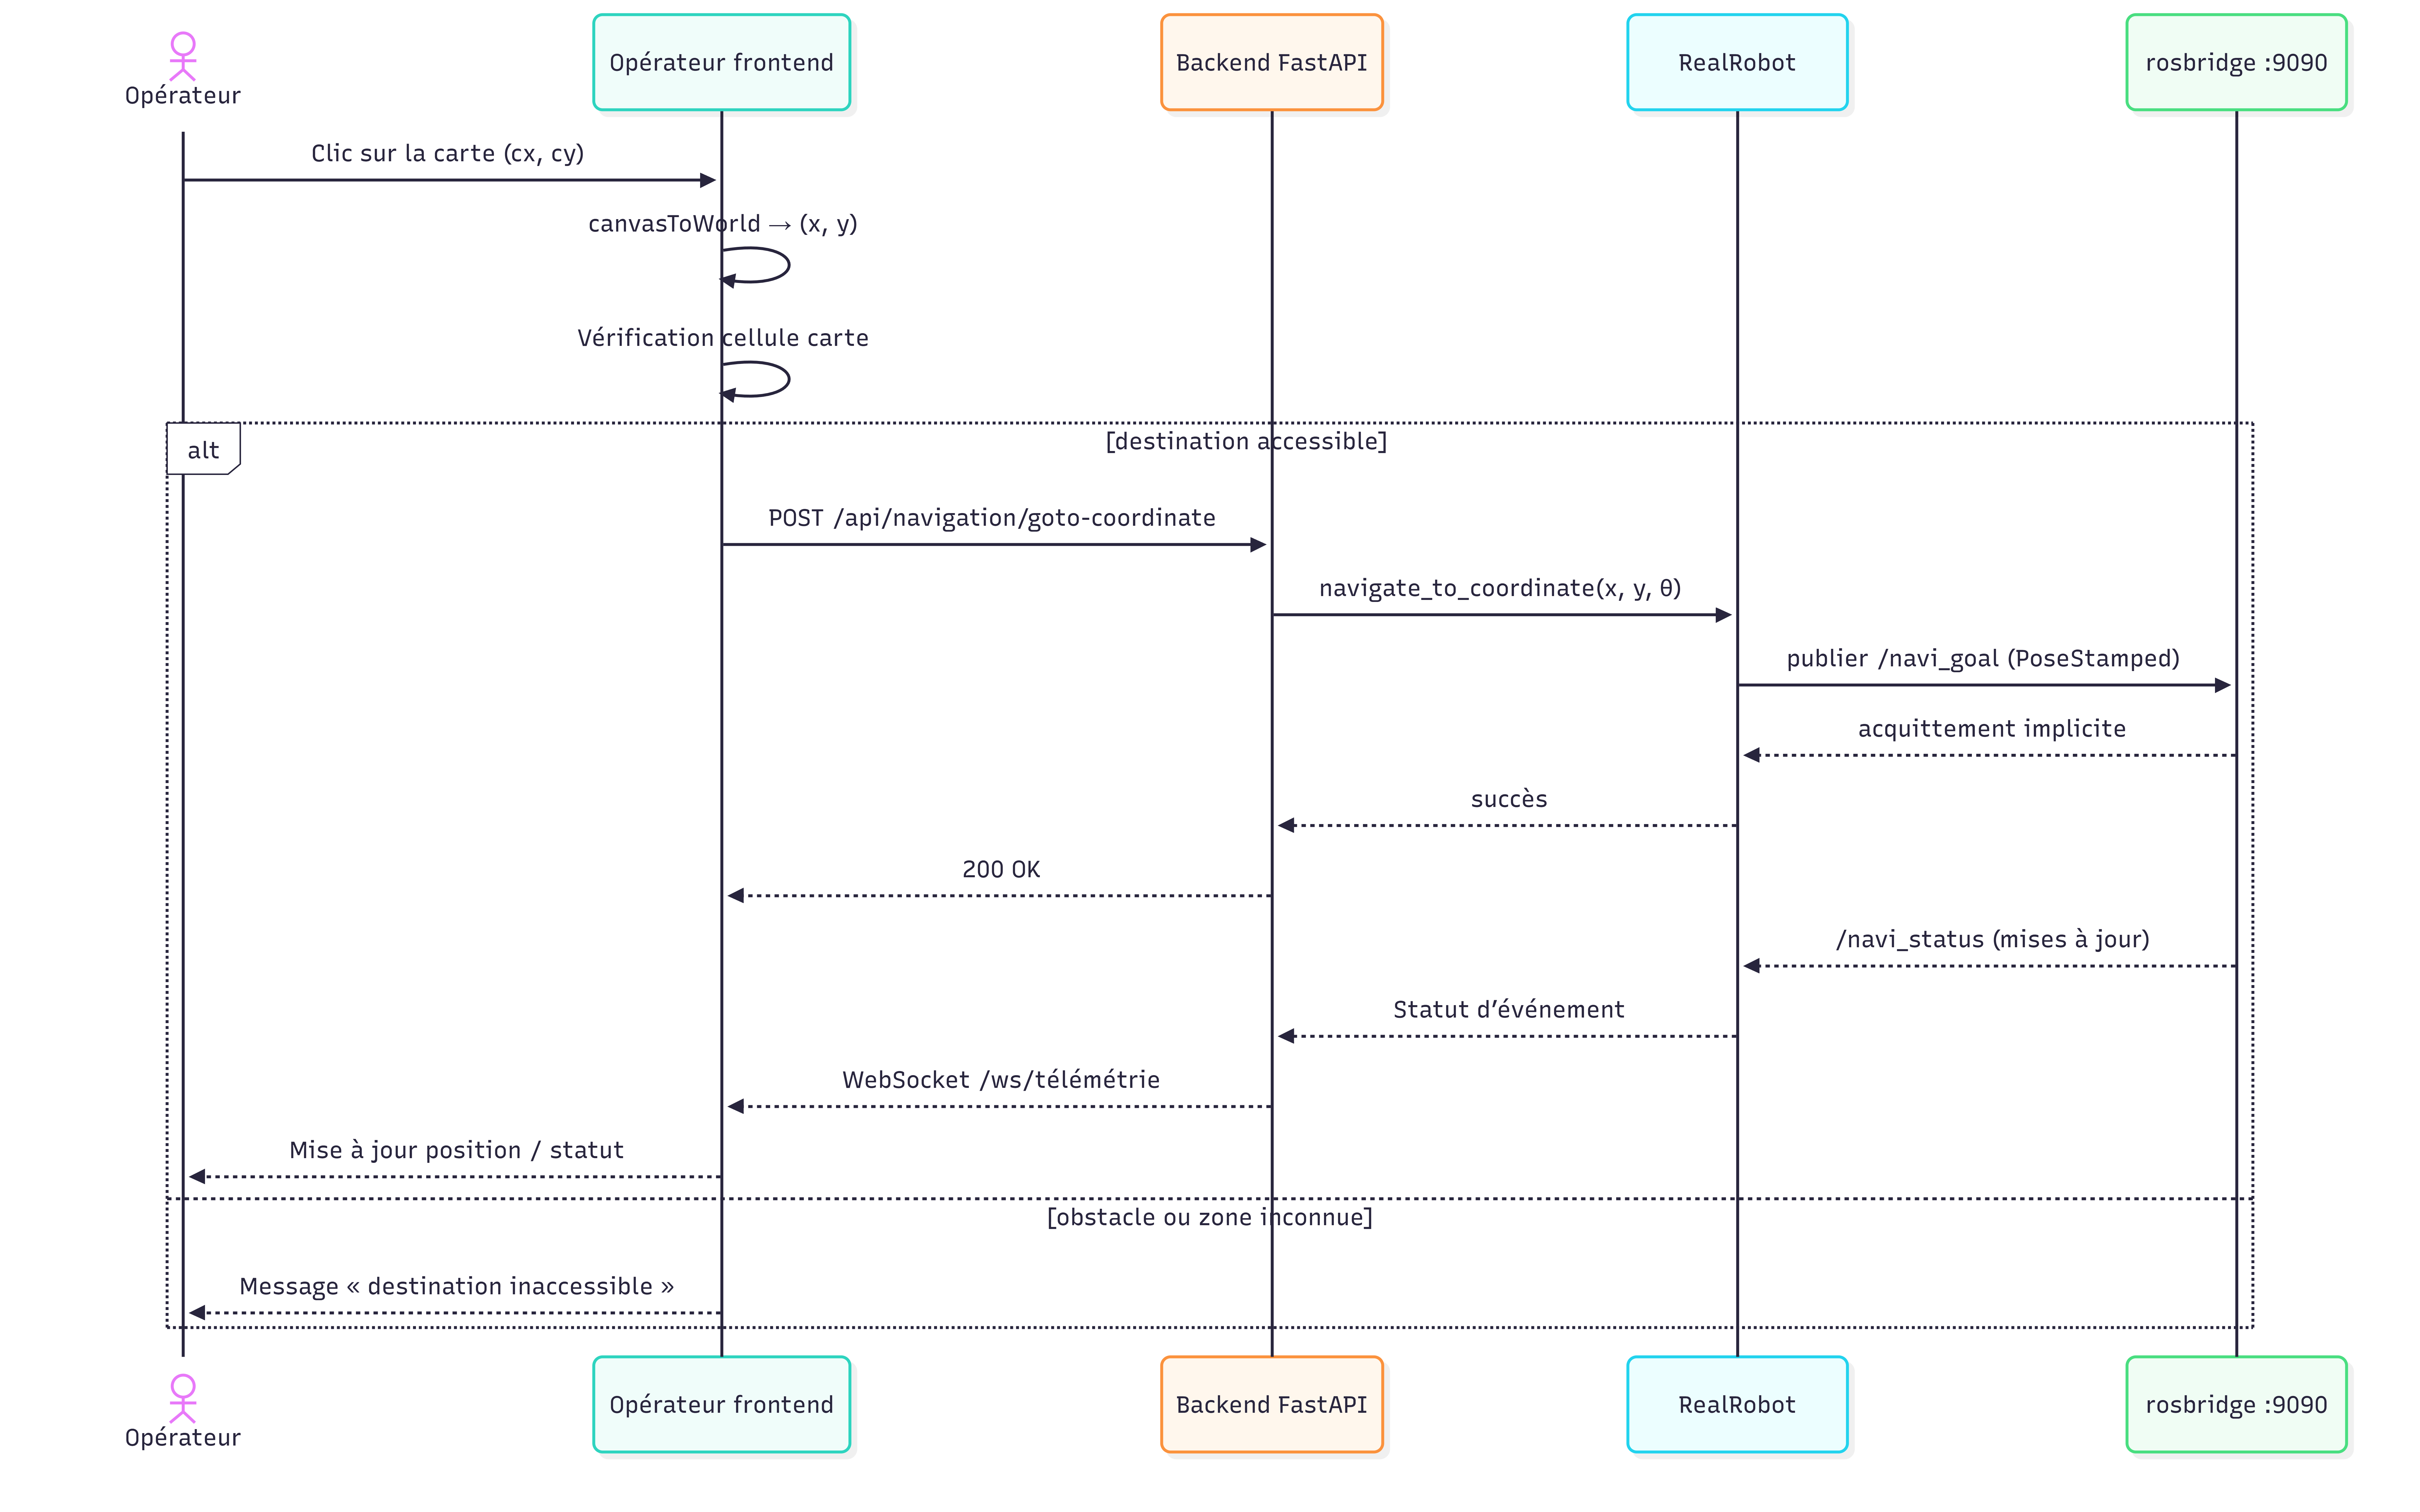
\includegraphics[width=0.85\textwidth]{diagramme/nce_navigation.png-2026-06-20-165623.png}
    \caption{Diagramme de séquence de la navigation vers un point sélectionné}
    \label{fig:diag_sequence}
\end{figure}

\subsection{Modèle des flux de communication}

\subsubsection*{Robot \texorpdfstring{$\leftrightarrow$}{<->} ROSBridge}

ROSBridge constitue la passerelle principale entre la plateforme CYBEL et
le système de navigation du robot. Les échanges reposent sur le protocole
WebSocket et permettent la réception des données de télémétrie,
l'abonnement aux topics ROS, l'appel de services, ainsi que l'envoi de
commandes de navigation et de mouvement.

\subsubsection*{ROSBridge \texorpdfstring{$\leftrightarrow$}{<->} Backend}

Le backend agit comme intermédiaire entre ROSBridge et les interfaces
utilisateur. Il collecte les informations provenant du robot, les traite
puis les redistribue vers les clients connectés. Il assure également la
gestion des commandes envoyées par les utilisateurs.

\subsubsection*{Backend \texorpdfstring{$\leftrightarrow$}{<->} Interfaces utilisateur}

Les interfaces communiquent avec le backend à travers des requêtes REST
pour les actions ponctuelles et des WebSockets pour les mises à jour
temps réel. Cette architecture garantit une supervision réactive et une
faible latence lors de l'affichage des données.

\subsubsection*{Backend \texorpdfstring{$\leftrightarrow$}{<->} Applications Android}

Les applications Android développées dans le cadre du projet permettent
d'étendre les fonctionnalités du système, notamment pour la synthèse
vocale, l'affichage du mode kiosque et les interactions avec la tablette
embarquée.

\subsection{Conclusion}

Ce chapitre a permis de présenter l'analyse fonctionnelle et la conception
générale du système CYBEL. Les besoins identifiés ont conduit à la
définition d'une architecture modulaire organisée autour d'un SDK robot,
d'une API centralisée et de plusieurs interfaces utilisateur. Les
différents diagrammes présentés permettent de visualiser les interactions
entre les acteurs et les composants du système ainsi que les flux de
communication mis en \oe uvre. Cette phase de conception constitue la base
des développements réalisés dans le chapitre suivant, consacré à la
méthodologie et à l'implémentation de la solution proposée.
\newpage
\section{Méthodologie et planification}
\label{chap:methodologie_planification}

La planification opérationnelle est un processus essentiel pour structurer et coordonner l’exécution des tâches dans une organisation ou un projet. 
Elle repose sur des méthodes rigoureuses, des applications pratiques et des outils spécialisés pour assurer une gestion efficace des ressources, des délais et des objectifs.

Ce glossaire définit les principaux concepts liés à la planification opérationnelle et explore les méthodes, applications et outils qui permettent d’optimiser son exécution.

Dans le cadre de notre stage, nous avons appliqué une démarche méthodique et structuré notre travail pour atteindre les objectifs fixés. 
Ce chapitre détaille notre mode de travail, la planification, les outils employés ainsi que les étapes concrètes de mise en œuvre.


\subsection{Mode de travail et organisation}
Dans le besoin d’un travail optimale, le mode de travail qui s’est avéré étant la plus optimale pour notre stage fut la répartition des tâches en optant sur nos points fort. 
Cette méthode nous auras permis de renforcer nos acquis sans pour autant rester dans notre zone de confort car malgré cette méthode de travail, il y a eu derrière un grand travail d’autonomie pour approfondir la documentation ou le développement des scripts Python présent au sein du compte GitHub \textbf{Claude20022002} sur lesquelles nous devions travailler.
Notre superviseur ainsi que tous les membres du laboratoire nous ont supervisés à travers des réunions, compte rendus journalier et hebdomadaire. Pour organiser notre travail, nous avons utilisé un planning détaillé et avons tenu des comptes rendus partagés sur Github où l'on présentait nos problèmes, hypothèses et solutions.


\subsection{Planning du travail}
Afin d'assurer une progression cohérente tout au long du stage et de respecter les objectifs fixés, un planning prévisionnel a été établi dès le début du projet sous la forme d'un diagramme de Gantt. Celui-ci a permis de répartir les différentes activités sur toute la durée du stage, d'identifier les dépendances entre les tâches et de suivre l'avancement du projet.
Le déroulement du projet a été organisé en quatre grandes phases successives.
La première phase, consacrée à la \textbf{connectivité}, avait pour objectif de comprendre l'architecture matérielle et réseau du robot. Cette étape a consisté à analyser la topologie du système, identifier les différents équipements présents sur le réseau et réaliser un balayage des ports afin de découvrir les services accessibles.
La deuxième phase concernait l'\textbf{investigation du système}. Durant cette étape, plusieurs travaux de rétro-ingénierie ont été réalisés afin d'identifier les mécanismes de communication utilisés par le robot. Les services ROS ont été explorés grâce à \texttt{rosapi}, les échanges MQTT ont été analysés afin de comprendre les commandes disponibles, tandis que le fonctionnement du système de synthèse vocale a été étudié à l'aide d'ADB et d'un pont de communication Android.
La troisième phase correspond au \textbf{développement de la plateforme CYBEL}. Cette étape a constitué la partie la plus importante du projet. Elle a conduit au développement d'un SDK Python permettant de communiquer avec le robot en mode simulé ou réel, à la réalisation du backend avec FastAPI et WebSocket, à la conception de l'interface web destinée aux opérateurs ainsi qu'au développement du moteur de visite guidée, du kiosque interactif destiné aux visiteurs et de la solution de déploiement sur la tablette Android via Termux.
Enfin, la quatrième phase est dédiée à la \textbf{validation du système}. Elle comprend les essais de navigation sur le robot réel, l'ajustement des coordonnées des différents points du parcours de visite, les tests d'intégration de l'ensemble des modules développés ainsi que la rédaction du rapport de stage et la préparation de la soutenance.
La Figure~\ref{fig:gantt} présente le planning global du projet et l'enchaînement des différentes phases de réalisation.

\begin{figure}[H]
    \centering
    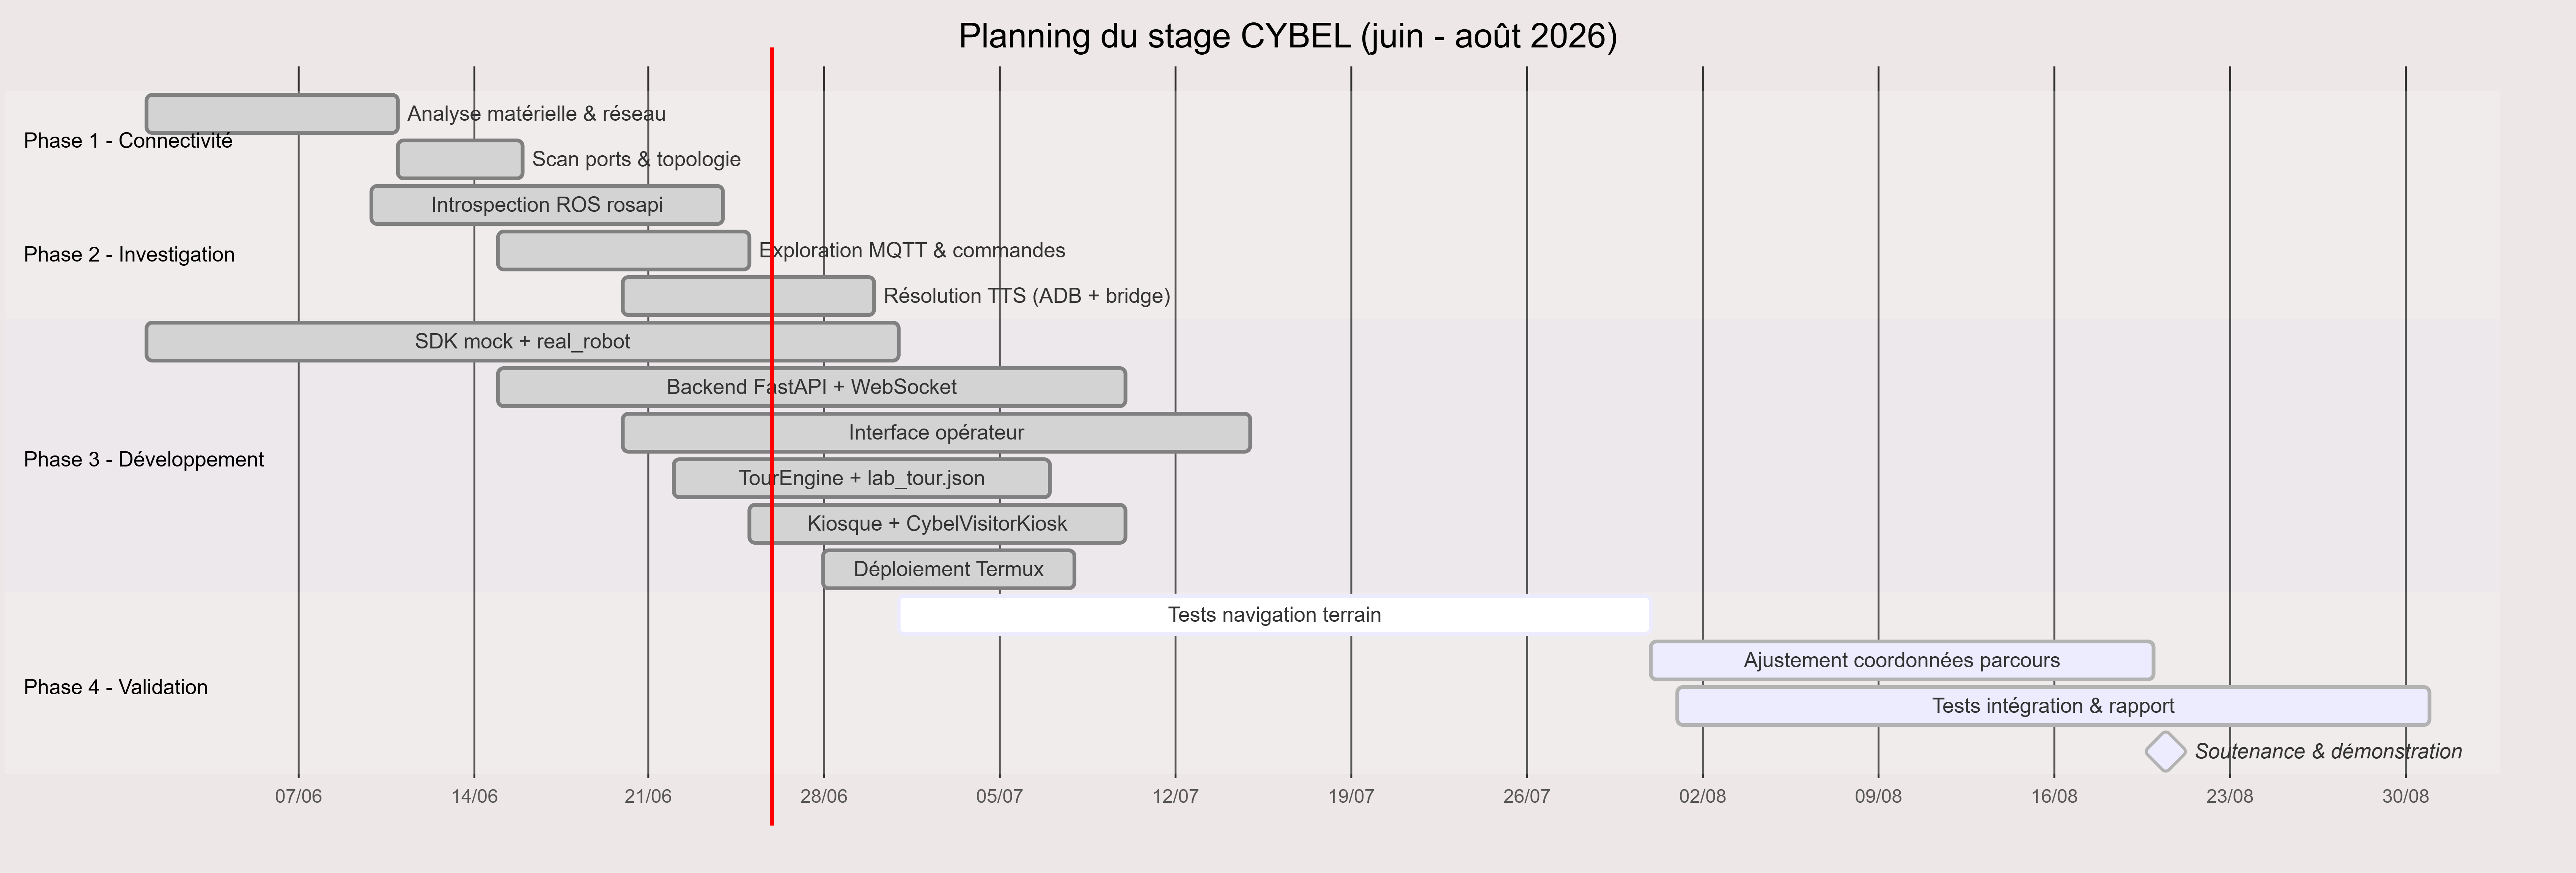
\includegraphics[width=\textwidth]{diagramme/diagramme-gantt-bg.png}
    \caption{Diagramme de Gantt du projet CYBEL}
    \label{fig:gantt}
\end{figure}

Comme le montre ce planning, plusieurs activités ont été menées en parallèle, notamment durant la phase de développement. Cette organisation a permis d'exploiter efficacement le temps disponible pendant les périodes où le robot n'était pas accessible, en poursuivant le développement de l'interface web, du backend ou des modules de simulation avant leur intégration sur le robot réel.


\subsection{Outils, Langage et Technologie utilisés}

\subsubsection{ROS}
\subsubsection{FastAPI}
\subsubsection{TypeScript}
\subsubsection{Android}
\subsubsection{ADB}
\subsubsection{ROS}

\subsection{Découverte du Robot CIOT TY1251D-03195 "CYBEL"}

\subsection{Proposition de documentation technique}

\subsection{Apports du stage}

\subsection{Difficultés rencontrées durant la phase d'investigation}

\subsection{Conclusion}
%================================================
% PARTIE 3 : RÉSULTATS ET VALIDATION
%================================================
\newpage
\section{Réalisation et implémentation}
\label{chap:realisation_implementation}

\subsection{Mise en place de l'environnement}

\subsection{Découverte et analyse du robot}

\subsection{Reverse Engineering du système}

\subsubsection{Analyse réseau}

\subsubsection{Identification des protocoles}

\subsubsection{Étude des commandes}

\subsection{Développement du backend CYBEL}

\subsection{Développement de l'application Android}

\subsection{Développement de l'interface Web}

\subsection{Mise en place du système TTS}

\subsection{Intégration des différents modules}

\subsection{Conclusion}
\newpage
\section{Validation, résultats et analyse critique}
\label{chap:Validation_result_ana_critique}

\subsection{Stratégie de validation}

\subsection{Scénarios de tests}

\subsection{Résultats obtenus}

\subsection{Indicateurs de performance}

Tableau avec :
Temps de réponse
Fiabilité
Stabilité des communications
Robustesse

\subsection{Contributions personnelles}

\subsection{Difficultés rencontrées et solutions apportées}

\subsection{Limites du projet}

\subsection{Perspectives d'amélioration}

\subsection{Conclusion}
%================================================
% CONCLUSION + BIBLIOGRAPHIE
%================================================
% Placeholder conclusion — fichier déplacé vers tex/ (à compléter)
\section*{\centering CONCLUSION GÉNÉRALE}
\addcontentsline{toc}{section}{CONCLUSION GÉNÉRALE}

% Le contenu original de `conclusion.tex` était vide. Complétez cette section
% avec la synthèse et les perspectives.

\newpage
\section*{\centering BIBLIOGRAPHIE}
\addcontentsline{toc}{section}{BIBLIOGRAPHIE}
\newpage
\section*{\centering WEBOGRAPHIE}
\addcontentsline{toc}{section}{WEBOGRAPHIE}

\begin{enumerate}
    \item Robot Web Tools. \textit{rosbridge\_suite}. Disponible sur :
    \url{https://github.com/RobotWebTools/rosbridge_suite}. Consulté le 20 juin 2026.

    \item Robot Web Tools. \textit{roslibjs}. Disponible sur :
    \url{https://github.com/RobotWebTools/roslibjs}. Consulté le 20 juin 2026.

    \item FastAPI. \textit{Documentation officielle}. Disponible sur :
    \url{https://fastapi.tiangolo.com}. Consulté le 18 juin 2026.

    \item Vite. \textit{Documentation officielle}. Disponible sur :
    \url{https://vitejs.dev}. Consulté le 18 juin 2026.

    \item Pydantic. \textit{Documentation officielle}. Disponible sur :
    \url{https://docs.pydantic.dev}. Consulté le 25 juin 2026.

    \item Mozilla Developer Network (MDN). \textit{Web Speech API}. Disponible sur :
    \url{https://developer.mozilla.org/en-US/docs/Web/API/Web_Speech_API}. Consulté le 21 juin 2026.

    \item Android Developers. \textit{TextToSpeech API}. Disponible sur :
    \url{https://developer.android.com/reference/android/speech/tts/TextToSpeech}. Consulté le 19 juin 2026.

    \item Android Developers. \textit{Android Debug Bridge (ADB)}. Disponible sur :
    \url{https://developer.android.com/tools/adb}. Consulté le 28 juin 2026.

    \item Termux Wiki. Disponible sur :
    \url{https://wiki.termux.com}. Consulté le 28 juin 2026.

    \item OWASP Foundation. \textit{OWASP Internet of Things Top 10}. Disponible sur :
    \url{https://owasp.org/www-project-internet-of-things/}. Consulté le 22 juin 2026.

    \item Mermaid. \textit{Documentation officielle}. Disponible sur :
    \url{https://mermaid.js.org}. Consulté le 25 juin 2026.

    \item Mermaid Live Editor. Disponible sur :
    \url{https://mermaid.live}. Consulté régulièrement pour la réalisation des diagrammes.

    \item Claudia LUSAMOTE KIMFUTA. \textit{Projet CYBEL}. Dépôt GitHub. Disponible sur :
    \url{https://github.com/Claude20022002/Projet-Stage-2026-Cybel}. Consulté quotidiennement en 2026.
\end{enumerate}
\newpage

\section*{ANNEXES}
\addcontentsline{toc}{section}{ANNEXES}

\subsection*{Annexe A — Captures d'écran}
\addcontentsline{toc}{subsection}{Annexe A — Captures d'écran}

% Remplacer chaque cadre par \includegraphics après ajout du fichier indiqué.

\begin{figure}[h!]
    \centering
    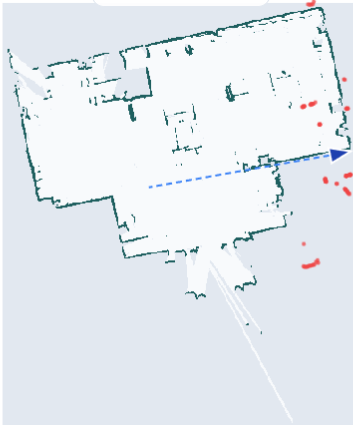
\includegraphics[width=0.8\textwidth]{captures_ecran/Capture1.png}
    \caption{Carte SLAM du laboratoire — interface opérateur
    (\texttt{captures\_ecran/Capture1.png})}
    \label{fig:annexe_carte}
\end{figure}

\begin{figure}[h!]
    \centering
    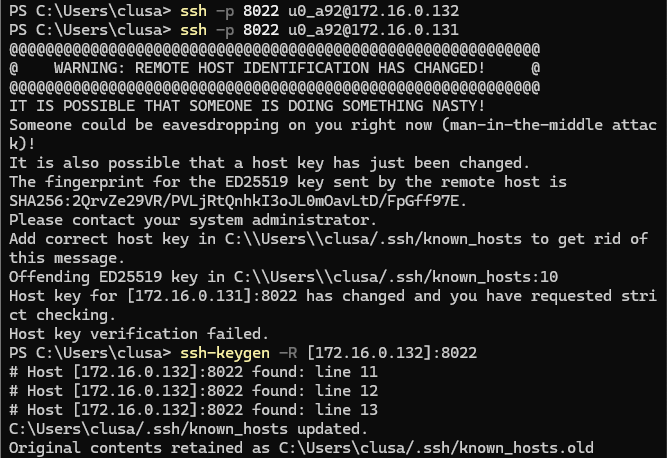
\includegraphics[width=0.8\textwidth]{captures_ecran/Capture2.png}
    \caption{Terminal — vérification de connectivité
    (\texttt{captures\_ecran/Capture2.png})}
    \label{fig:annexe_terminal}
\end{figure}

\begin{figure}[h!]
    \centering
    \fbox{\parbox{0.75\textwidth}{\centering\vspace{2.5cm}
    \textit{Capture à insérer}\\[0.3cm]
    \texttt{captures\_ecran/dashboard\_operateur.png}\vspace{2.5cm}}}
    \caption{Dashboard opérateur — mode robot réel \textit{(à insérer)}}
    \label{fig:annexe_dashboard}
\end{figure}

\begin{figure}[h!]
    \centering
    \fbox{\parbox{0.75\textwidth}{\centering\vspace{2.5cm}
    \textit{Capture à insérer}\\[0.3cm]
    \texttt{captures\_ecran/panneau\_visite.png}\vspace{2.5cm}}}
    \caption{Panneau visite guidée — page Visite \textit{(à insérer)}}
    \label{fig:annexe_visite}
\end{figure}

\begin{figure}[h!]
    \centering
    \fbox{\parbox{0.75\textwidth}{\centering\vspace{2.5cm}
    \textit{Capture à insérer}\\[0.3cm]
    \texttt{captures\_ecran/kiosque\_accueil.png}\vspace{2.5cm}}}
    \caption{Kiosque visiteur — écran d'accueil FR \textit{(à insérer)}}
    \label{fig:annexe_kiosque_accueil}
\end{figure}

\begin{figure}[h!]
    \centering
    \fbox{\parbox{0.75\textwidth}{\centering\vspace{2.5cm}
    \textit{Capture à insérer}\\[0.3cm]
    \texttt{captures\_ecran/kiosque\_running.png}\vspace{2.5cm}}}
    \caption{Kiosque visiteur — visite en cours \textit{(à insérer)}}
    \label{fig:annexe_kiosque_running}
\end{figure}

\begin{figure}[h!]
    \centering
    \fbox{\parbox{0.75\textwidth}{\centering\vspace{2.5cm}
    \textit{Capture à insérer}\\[0.3cm]
    \texttt{captures\_ecran/erreur\_604.png}\vspace{2.5cm}}}
    \caption{Erreur de navigation 604 sur tablette \textit{(à insérer)}}
    \label{fig:annexe_erreur_604}
\end{figure}

\begin{figure}[h!]
    \centering
    \fbox{\parbox{0.75\textwidth}{\centering\vspace{2.5cm}
    \textit{Capture à insérer}\\[0.3cm]
    \texttt{captures\_ecran/apk\_tablette.png}\vspace{2.5cm}}}
    \caption{Application \texttt{CybelVisitorKiosk} sur tablette \textit{(à insérer)}}
    \label{fig:annexe_apk}
\end{figure}

\subsection*{Annexe B — Dépôt source du projet}
\addcontentsline{toc}{subsection}{Annexe B — Dépôt source du projet}

\begin{itemize}
    \item \textbf{Dépôt principal CYBEL} (branche \texttt{main}) :\\
    \url{https://github.com/Claude20022002/Projet-Stage-2026-Cybel}
    \item \textbf{Branche chatbot} (G. Khalifi) :\\
    \url{https://github.com/Claude20022002/Projet-Stage-2026-Cybel/tree/chatbot-cybel-projet-2026}
\end{itemize}

\subsection*{Annexe C — Commandes utiles}
\addcontentsline{toc}{subsection}{Annexe C — Commandes utiles}

\begin{lstlisting}[style=terminal, language=bash, caption={Commandes PC (PowerShell)}]
# Verification reseau
ping 10.42.0.1
python scripts\robot_status.py

# Lancement developpement
python scripts\dev.py

# Tests unitaires (78 tests)
python -m pytest tests/ -v

# TTS test (USB branche)
adb shell am broadcast -n com.cybel.ttsbridge/.SpeakReceiver ^
  -a com.cybel.ttsbridge.SPEAK --es text "Test HESTIM"

# Deploiement tablette
python scripts\deploy_termux.py --skip-kiosk-build --lite-only --host <IP>
\end{lstlisting}

\begin{lstlisting}[style=terminal, language=bash, caption={Commandes Termux (tablette)}]
cd ~/cybel/scripts/termux
./stop_cybel.sh && ./start_cybel.sh
curl http://127.0.0.1:8000/api/health
\end{lstlisting}

\subsection*{Annexe D — Extraits de code significatifs}
\addcontentsline{toc}{subsection}{Annexe D — Extraits de code significatifs}

\paragraph{D.1 — Annulation de navigation (\texttt{sdk/real\_robot.py}).}

\begin{verbatim}
async def _cancel_navigation(self) -> None:
    for args in [{"command": "stop"}, ...]:
        await self._client.call_service(
            ROS_SERVICES["poi"], args, timeout=3.0)
    await call_service_first(self._client, ...)
    await self._publish_velocity(0.0, 0.0)
\end{verbatim}

\paragraph{D.2 — Publication d'un objectif de navigation.}

\begin{verbatim}
await self._client.publish(ROS_TOPICS["navi_goal"], {
    "header": {"frame_id": "map"},
    "pose": {
        "position": {"x": x, "y": y, "z": 0.0},
        "orientation": {"z": sin(theta/2), "w": cos(theta/2)},
    },
})
\end{verbatim}

\paragraph{D.3 — Structure d'un arrêt (\texttt{data/lab\_tour.json}).}

\begin{verbatim}
{
  "id": "cnc_router",
  "equipment_fr": "Routeur CNC",
  "x": -8.38, "y": 1.45, "theta": 0.88,
  "speech_fr": "Le routeur CNC permet d'usiner...",
  "dwell_seconds": 12
}
\end{verbatim}

\subsection*{Annexe E — Diagrammes détaillés}
\addcontentsline{toc}{subsection}{Annexe E — Diagrammes détaillés}

Sources Mermaid dans \texttt{docs/Sujet de stage/diagrammes/} du dépôt CYBEL.
Remplacer chaque cadre par \texttt{\textbackslash includegraphics} après export PNG.

\begin{figure}[h!]
    \centering
    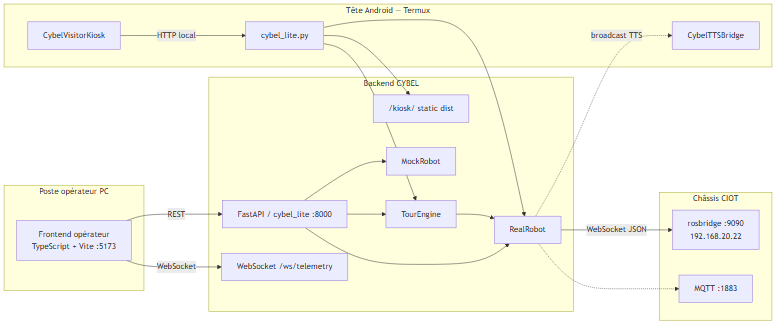
\includegraphics[width=0.85\textwidth]{diagramme/diagramme_composant.png}
    \caption{Diagramme de composants
    (\texttt{diagramme/diagramme\_composant.png})}
    \label{fig:annexe_composants}
\end{figure}

\begin{figure}[h!]
    \centering
    \fbox{\parbox{0.75\textwidth}{\centering\vspace{2.5cm}
    \textit{Diagramme à insérer}\\[0.3cm]
    \texttt{diagramme/architecture\_couches.png}\vspace{2.5cm}}}
    \caption{Architecture en couches \textit{(à insérer)}}
    \label{fig:annexe_archi_couches}
\end{figure}

\begin{figure}[h!]
    \centering
    \fbox{\parbox{0.75\textwidth}{\centering\vspace{2.5cm}
    \textit{Diagramme à insérer}\\[0.3cm]
    \texttt{diagramme/topologie\_reseau.png}\vspace{2.5cm}}}
    \caption{Topologie réseau du robot \textit{(à insérer)}}
    \label{fig:annexe_topologie}
\end{figure}

\begin{figure}[h!]
    \centering
    \fbox{\parbox{0.75\textwidth}{\centering\vspace{2.5cm}
    \textit{Diagramme à insérer}\\[0.3cm]
    \texttt{diagramme/sequence\_lab\_tour.png}\vspace{2.5cm}}}
    \caption{Séquence — visite guidée laboratoire \textit{(à insérer)}}
    \label{fig:annexe_seq_tour}
\end{figure}

\begin{figure}[h!]
    \centering
    \fbox{\parbox{0.75\textwidth}{\centering\vspace{2.5cm}
    \textit{Diagramme à insérer}\\[0.3cm]
    \texttt{diagramme/sequence\_tts.png}\vspace{2.5cm}}}
    \caption{Séquence — synthèse vocale (TTS) \textit{(à insérer)}}
    \label{fig:annexe_seq_tts}
\end{figure}

\subsection*{Annexe F — Documentation technique complémentaire}
\addcontentsline{toc}{subsection}{Annexe F — Documentation technique complémentaire}

\begin{table}[h!]
\centering
\caption{Index de la documentation technique CYBEL}
\begin{tabular}{|p{5cm}|p{8cm}|}
\hline
\textbf{Document} & \textbf{Chemin dans le dépôt} \\
\hline
README projet & \texttt{README.md} \\
\hline
Guide interface opérateur & \texttt{docs/INTERFACE.md} \\
\hline
Pont TTS & \texttt{docs/TTS\_BRIDGE.md} \\
\hline
Kiosque visiteur & \texttt{docs/VISITOR\_KIOSK.md} \\
\hline
Déploiement Termux & \texttt{docs/TERMUX\_DEPLOY.md} \\
\hline
Connexion robot & \texttt{docs/ROBOT\_CONNECTION.md} \\
\hline
Procédure terrain & \texttt{docs/labo/TERRAIN.md} \\
\hline
\end{tabular}
\end{table}

\end{document}